In this chapter we present some concepts related to the intersection of the two areas:  computer science methods used to solve electrical engineering problems; in this case, the use of formal verification methodology to perform automated verification and optimal sizing of stand-alone solar PV systems.

First, we introduce the concept of formal verification as background to understanding how a methodology that performs (mainly) bug detection can be used to validate a design sizing or to obtain an optimal solution of PV systems.

And secondly, how a solar PV system can be modeled in order to be validated or optimized by formal verification methodology.

%%%%%%%%%%%%%%%%%%%%%%%%%%%%%%%%%%%%%%%%%%%%%%%%%%%%%%%%
\section{Formal Methods, Formal Design and Formal Verification}
%%%%%%%%%%%%%%%%%%%%%%%%%%%%%%%%%%%%%%%%%%%%%%%%%%%%%%%%

Formal methods are system design techniques that use rigorously specified mathematical models to validate systems, most notably (and known for) software and hardware systems~\cite{Collins98}. In contrast to other design systems, formal methods use mathematical proof as a complement to system testing in order to ensure correct behavior. With increasing scale and complexity, when safety becomes a more important issue, the formal approach to system design offers a better level of insurance.

Formal methods differ from other design systems through the use of formal verification schemes; the basic principles of the system must be proven correct before they are accepted~\cite{Bowen93}. Traditional system design has used extensive testing to verify behavior, but testing is capable of only finite conclusions. Dijkstra and others have demonstrated that tests can only show the situations where a system will not fail, but can say nothing about the behavior of the system outside of the testing scenarios~\cite{Bentley99}. In contrast, a theorem once proven true remains true.

Prior to the 1980s, mainly deductive verification was used as the formal method, with the use of axioms and proving rules to demonstrate the correctness of the system. The original focus was to verify critical systems based on the premise that if the system is important, time must be spent to verify it~\cite{Lowry1998}. Originally, formal methods were performed by hand.

It is worth pointing out that formal verification does not avoid the need for testing~\cite{Bowen95}. Formal verification can not correct bad assumptions in the design, but it can help to identify errors in reasoning which would otherwise be left unverified. In several cases, engineers have reported finding flaws in systems following a formal review of their designs~\cite{Kling95}.

A formal design can be summarized as a three step process, as described below~\cite{Collins98}:

\begin{itemize}
\item Formal Specification. During the formal specification phase, the engineer rigorously defines a system using a modeling language. Modeling languages are fixed grammars which allow users to model complex structures from predefined types (that are rigorously defined). This process of formal specification is similar to the process of converting a word problem into algebraic notation and helps researchers and engineers to clearly define their problems, goals and solutions. Several engineers who have used formal specifications claim that the clarity that this stage produces is a benefit in itself~\cite{Kling95}.
\item Verification. As stated above, formal methods differ from other specification systems by their heavy emphasis on provability and correctness. In building a system using formal specification, the designer is actually developing a set of theorems about his system. By proving these theorems correct, the formal verification ensures that the modeled system has an intended behavior. Verification is a difficult process, largely because even the simplest system has several dozen theorems, each of which has to be proven. Given the demands of complexity and Moore's law, almost all formal systems use an automated theorem proving tool of some form~\cite{Collins98}. That is the origin of 'automated verification' definition. These tools can prove simple theorems, verify the semantics of theorems, and provide assistance for verifying more complicated proofs, with feedback about the trace of the error (in order to correct the system and the specification of it).
\item Implementation. Once the model has been specified and verified, it is implemented by converting the specification into code.

\end{itemize}

%Formal methods are viewed with a certain degree of suspicion. While formal methods research has been progressing since 1960's, formal methods are only being slowly accepted by engineers. There are several reasons for this, but most of the problems seem to be a result of misapplication. Most formal systems are extremely descriptive and all-encompassing, modeling languages have generally been judged by their capacity to model anything. Unfortunately, these same qualities make formal methods very difficult to use, especially for engineers untrained in the type theory needed for most formal systems.[Bowen93]
%
%Conversely, it is apparent that some form of formal specification is necessary: complex systems require formal models. In addition,the mathematics required for formal methods is becoming a more prominent fixture of engineering curricula, engineering schools in Europe are already requiring courses in VDM, Z and similar formal specifications. Ultimately, formal methods will acquire some form of acceptance, but compromises will be made in both directions: formal methods will become simpler and formal methods training will become more common.
%
%Key Concepts
%Provability And Automated Verification
%Formal methods are distinguished from other specification systems by their emphasis on correctness and proof, which is ultimately another measure of system integrity. Proof is a complement, not a substitute, for testing. Testing is an important part of guaranteeing any system's fitness, but it is finite. Testing cannot demonstrate that a system operates properly; it can only demonstrate that the system works for the tested cases. Because testing cannot demonstrate that the system should work outside the tested cases, formal proof is necessary.
%
%Formally proving computer systems is not a new idea. Knuth and Dijkstra have written extensively on the topic, although their methods of proof are based on the traditional mathematical methods. In pure sciences, proofs are verified through extensive peer review before publication. Such techniques are time-intensive and less than perfect; it isn't unusual for a published proof to contain a flaw. Given the cost and time requirements of systems engineering, traditional proving techniques are not really applicable.
%
%Because of the costs of hand verification, most formal methods use automated theorem proving systems to verify their designs. Automated theorem provers are best described as mathematical CAD tools: they can prove simple propositions and automatically and provide assistance for verifying more complex theorems.
%
%Benefits Of Formal Models
%Formal methods offer additional benefits outside of provability, and these benefits do deserve some mention. However, most of these benefits are available from other systems, and usually without the steep learning curve that formal methods require.
%
%Discipline: By virtue of their rigor, formal systems require an engineer to think out his design in a more thorough fashion. In particular, a formal proof of correctness is going to require a rigorous specification of goals, not just operation. This thorough approach can help identify faulty reasoning far earlier than in traditional design.[Bowen95]
%The discipline involved in formal specification has proved useful even on already existing systems. Engineers using the PVS system, for example, reported identifying several microcode errors in one of their microprocessor designs.[Miller95]
%
%Precision: Traditionally, disciplines have moved into jargons and formal notation as the weaknesses of natural language descriptions become more glaringly obvious. There is no reason that systems engineering should differ, and there are several formal methods which are used almost exclusively for notation.[Bowen93]
%For engineers designing safety-critical systems, the benefits of formal methods lie in their clarity. Unlike many other design approaches, the formal verification requires very clearly defined goals and approaches. In a safety critical system, ambiguity can be extremely dangerous, and one of the primary benefits of the formal approach is the elimination of ambiguity.[Kling94].
%
%Weaknesses Of Formal Methods
%: Bowen points out that formal methods are generally viewed with suspicion by the professional engineering community, and the propensity of tentative case studies and advocacy papers for the formal approach would seem to support his thesis [Bowen93]. There are several reasons why formal methods are not used as much as they might be, most stemming from overreaching on the part of formal methods advocates.
%Expense:Because of the rigor involved, formal methods are always going to be more expensive than traditional approaches to engineering. However, given that software cost estimation is more of an art than a science, it is debatable exactly how much more expensive formal verification is. In general, formal methods involve a large initial cost followed by less consumption as the project progresses; this is a reverse from the normal cost model for software development.[Bowen93]
%
%Limits Of Computational Models:While not a universal problem, most formal methods introduce some form of computational model, usually hamstringing the operations allowed in order to make the notation elegant and the system provable. Unfortunately, these design limitations are usually considered intolerable from a developer's perspective.
%An excellent example comes from SML. Statements of proof in SML depend on a purely functional programming model: all data is passed through the parameter/return mechanism of a function, no side effect alterations, modifications of global variables or the like is allowed [Paulson96]. Handling side effects and other aberrancies are a requirement for any system involving input, network operations or other systems which require interrupts, meaning that SML's model is, to some extent, broken.
%
%Usability:Traditionally, formal methods have been judged on the richness of their descriptive model. That is, 'good' formal methods have described a wide variety of systems, and 'bad' formal methods have been limited in their descriptive capacities. While an all-encompassing formal description is attractive from a theoretical perspective, it invariably involved developing an incredibly complex and nuanced description language, which returns to the difficulties of natural language. Case studies of full formal methods often acknowledge the need for a less all-encompassing approach.[Miller95]
%Arguably, many of these failures can be attributed to overreaching on the part of formal methods advocates. This reasoning has led to the lightweight approach to formal specification.
%
%The Lightweight Approach
%The flaws in formal specifications have been heavily focused on in the past few years, leading to several alternate approaches. The traditional view of formal methods as all-encompassing highly abstracted schemes has led to formal methods being all-encompassing, extremely rigorous, and very expensive. While theoretically appealing, formal methods have generally been ignored by engineers in the field.
%The lightweight approach to formal design recognizes that formal methods are not a panacea: there are areas where formal methods are useful, and areas where a formal specification will accomplish nothing. In a lightweight design, formal methods are used in specific locations, and different formal methods may be used in different subsystems, ideally playing to the strengths of each method [Easterbrook 98]. In such a system, Petri Nets might be used to describe the communications protocol, and a LARCH system might be used to model the data storage. For other parts of the system, formal specifications might be avoided entirely: for example, the user interface may be refined using a rapid prototyping system and client interviews.
%
%The lightweight approach is a traditional engineering compromise, and there is a tradeoff. As formal methods become more common, engineers will have to learn type theory, modern algebra and proof techniques. Ultimately, engineers will have to think more like mathematicians.

%%%%%%%%%%%%%%%%%%%%%%%%%%%%%%%%%%%%%%%%%%%%%%%%%%%%%%%%
\section{Project Validation, Automated Verification and Synthesis Using Model Checking}
\label{sec:AutomatedVerification}
%%%%%%%%%%%%%%%%%%%%%%%%%%%%%%%%%%%%%%%%%%%%%%%%%%%%%%%%

%\section{Automated Verification }
It is necessary to keep in mind that validation is the process of determining whether a design meets the needs of the user, whereas verification is the process of determining whether a design meets a set of requirements, specifications, and regulations.  

If the requirements, specifications, and regulations are given in a formal language, then it may be possible to automate verification.  

Simulation may also be used for validation, but it raises more problems for verification. In order to use simulation for verification, it is necessary to ensure adequate coverage of operating conditions, scenarios, and system inputs. Testing can also be used for validation, but for the same reasons, it too raises problems for verification.
 
According to \cite{Clarke2008}, verification procedure is an intelligent exhaustive search of the state space of the design. In addition, according to \cite{Forejt2011}, formal verification is a systematic approach that applies mathematical reasoning to obtain guarantees about the correctness of a system. One successful method in this domain is model checking.

\subsection{Model Checking}
  
Model checking is an automatic verification technique, as defined by \cite{Clarke2008}. Model checking was originally developed for reasoning about finite state of concurrent systems, though nowadays it is mainly used for hardware and software verification, but can be applied to any kind of system. 

The process of model checking can be divided in three components: modeling, specification, and verification method. 

\begin{itemize}
\item In modeling, a model (usually mathematical) of the system is created; 
\item In specification, usually a list of properties to be satisfied by the system is established, i.e., the requirements, such as reliability to performance, for example; 
\item It is expressed usually in temporal logic form ($CTL$); 
\item The model checking is the verification method itself. 
\end{itemize}

The model checking algorithm can be described as:  

\begin{itemize}
\item Given the model $ 'M' $ and a $CTL$ formula $ \phi $ as input;  
\item The moodel checking algorithm provides all the states of model $ M $ which satisfy $ \phi $;  
\item It returns $YES$ if $ \phi $ is $TRUE$, or returns $NO$ if $ \phi $ is $FALSE$.  

\end{itemize}
Specifically, in the case of $ \phi $ being $FALSE$, the algorithm returns a counterexample that is useful as a system diagnostic, in order to discover in which situation the model has been violated. \cite{Clarke2008} considers this to be the most important advantage of model checking.  
 
Model checking presents several other advantages: proofs are not needed (the algorithm is not a deductive procedure); there is no problem with partial specifications of the system, logics can easily express many concurrency properties; it is fast (compared to other rigorous methods such as interactive theorem proving). However, there is one major disadvantage in model checking: the state explosion problem. 

The model checking problem can be defined as shown in \cite{Clarke2008}: 

\begin{itemize}
\item Let $M$ be a Kripke structure (i.e., a state transition graph);
\item $f$ be the specification in temporal logic (a formula);
\item Find all states $s$ of $M$ such that $M , s \models f$
\end{itemize}

Fig. \ref{fig:modelcheckstruc} shows the structure of a typical model checking system. A preprocessor extracts a state transition graph from a system (program or circuit).

\begin{figure}[h]
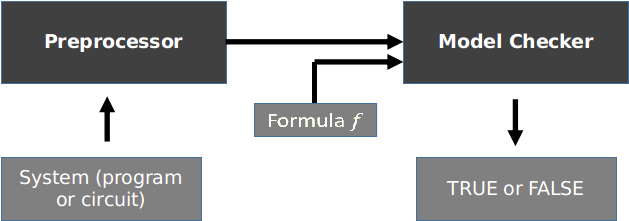
\includegraphics[width=0.8\textwidth]{modelcheckstruc}
\centering
\caption{Model Checker structure. Source: \cite{Clarke2008}.}
\label{fig:modelcheckstruc}
\end{figure}

Here it is worth mentioning that the term "model" is not used here with its dictionary definition. In other words, the problem is not dealing with an abstraction of the actual system under study. Therefore, model can be defined as a (usually finite-state) description of the system to be analyzed.

The Fig. \ref{fig:systemverif} shows the process of converting a real system to a model in order to be verified by model checking. 

\begin{figure}[h]
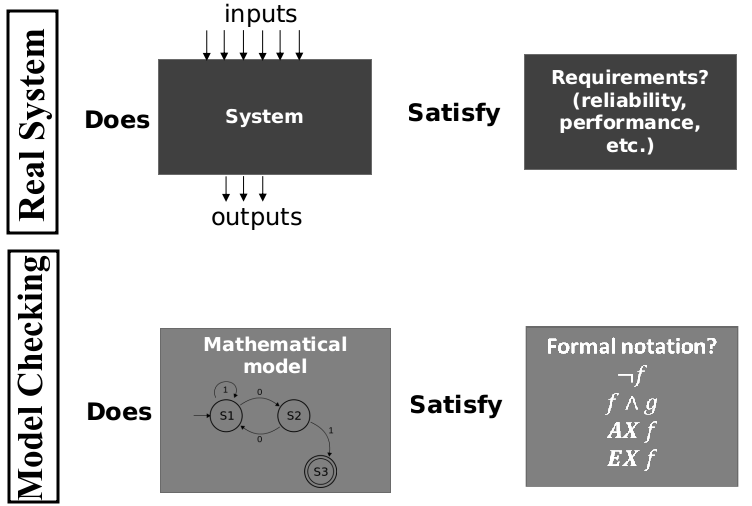
\includegraphics[width=0.8\textwidth]{systemverif3}
\centering
\caption{From real system verification to model checking. Source: adapted from \cite{Clarke2008}.}
\label{fig:systemverif}
\end{figure}

In order to solve the problem of state explosion, many different techniques have been developed over the last decades. One of the most promising is Bounded Model Checking (BMC). 

BMC is a method that checks the model up to a given point in the path length. The BMC algorithms traverse a finite state machine for a fixed number of steps, $k$, and check whether violation occurs within this bound. It uses fast SAT solvers, where SAT means satisfiability. 

A SAT problem, as defined by \cite{Clarke2008}, is a problem of determining if there are certain conditions or interpretations that satisfy a given Boolean expression. SAT solvers are used in BMC, such that if there is some Boolean function, the solver would search the model for conditions (value of variables) that would make the formula $TRUE$. If the SAT Solver finds a substitution for the formula/function then the substitute induces a counterexample.  

%%CBMC is considering the best-known model verification tool to validate code in ANSI-C and C++, as can be seen in \cite{Kroening}. 
%
%ESBMC is a context-bounded model checker for embedded C/C++ software based on Satisfiability Modulo Theories (SMT) solver, which can use CBMC as front-end.  
The use of SMT, instead of Boolean Satisfiability SAT from the original BMC, comes as an alternative to overcome limitations of the system's modeling, especially considering that the complexity of these is increasing and the SMT method has a higher level and richer theories than the SAT to represent the models. 

%Although simulation and testing explore possible behaviors and scenarios of a given system, they leave open the question of whether unexplored trajectories may contain a flaw~\cite{ClarkeHV18}. Formal verification conducts an exhaustive exploration of all possible behaviors; when a design is said to be ``correct'' by a formal verification method, it implies that all behaviors have been explored; questions regarding adequate coverage or missed behavior becomes irrelevant~\cite{Clarke2012}. Formal verification is a systematic approach that applies mathematical reasoning to obtain guarantees about the correctness of a system; one successful method in this domain is model checking~\cite{Clarke2012}. 

In this study we will evaluate three state-of-the-art model checkers to formally verifying and synthesize PV designs w.r.t. user requirements. In addition, other solvers will be evaluated, according to the feature of each model checker.

%%%%%%%%%%%%%%%%%%%%%%%%%%%%%%%%%%%%%%%%%%%%%%%%%%%%%%%%
\subsection{CBMC}
%%%%%%%%%%%%%%%%%%%%%%%%%%%%%%%%%%%%%%%%%%%%%%%%%%%%%%%%

The C Bounded Model Checker (CBMC) falsifies assertions in C programs or proves that they are safe if a completeness threshold is given~\cite{Kroening}. CBMC implements a bit-precise translation of a C program, annotated with assertions and with loops unrolled up to a given depth, into a logical formula. If the formula is satisfiable, then a failing execution that leads to a violated assertion exists~\cite{Kroening}. 

CBMC's verification flow can be summarized in three stages: 

\begin{itemize}
\item Front-end: scans, parses and type-checks C code; it converts control flow elements, such as \textit{if} or \textit{switch} statements, loops and jumps, into equivalent guarded \textit{goto} statements, thus aiming to reduce verification effort; 
\item Middle-end: performs symbolic execution by eagerly unwinding loops up to a fixed bound, which can be specified by the user on a per-loop basis or globally, for all loops and finally; 
\item Back-end: supports SAT and SMT solvers to discharge verification conditions.
\end{itemize}

Specifically, CBMC comes with a built-in solver for bit-vector formulas that is based on MiniSat. We used this solver during the experimentation in this Ph.D thesis~\cite{Kroening}.

%%%%%%%%%%%%%%%%%%%%%%%%%%%%%%%%%%%%%%%%%%%%%%%%%%%%%%%%
\subsection{ESBMC}
\label{sec:ESBMC}
%%%%%%%%%%%%%%%%%%%%%%%%%%%%%%%%%%%%%%%%%%%%%%%%%%%%%%%%

The Efficient SMT-based Bounded Model Checker (ESBMC) is a bounded and unbounded model checker for C~\cite{esbmc2018,GadelhaMCN19}, C++~\cite{RamalhoFSMC013}, Qt~\cite{MonteiroGCF17}, and CUDA~\cite{PereiraASMMFC17} programs, which supports the verification of LTL properties with bounded traces~\cite{DBLP:journals/sosym/MorseCN015}. 

ESBMC's verification flow can be summarized in three stages: 

\begin{itemize}
\item A front-end that can read and compile C code, where the system's formal specification is first handled; 
\item Preprocessing steps deal with code representation, control flow and unwinding of loops, and model simplification, thereby aiming to reduce verification effort; and finally 
\item The SMT solving stage, where all constraints and properties of the system are encoded into SMT and checked for satisfiability.
\end{itemize}
 
ESBMC exploits the standardized input language of SMT solvers (SMT-LIB\footnote{http://smtlib.cs.uiowa.edu/} logic format) to make use of a resource called \textit{assertion stack}~\cite{Morse2015}. This enables ESBMC, and the respective solver, to learn from previous checks, thus optimizing the search procedure and potentially eliminating a large amount of formula state space to be searched, because it solves and disregards data during the process, incrementally. This technique is called 'incremental SMT'~\cite{DBLP:journals/fac/SchrammelKBMTB17} and allows ESBMC to reduce the memory overhead, mainly when the verified system is complex and the computing platform does not have a large amount of memory to deal with the entire design space state. ESBMC in 'incremental SMT' uses only the Z3 solver~\cite{DeMoura}.

%%%%%%%%%%%%%%%%%%%%%%%%%%%%%%%%%%%%%%%%%%%%%%%%%%%%%%%%
\subsection{CPAchecker}
%%%%%%%%%%%%%%%%%%%%%%%%%%%%%%%%%%%%%%%%%%%%%%%%%%%%%%%%

Automatic program verification requires a choice between precision and efficiency. The more precise a method, the fewer false positives it will produce, but also the more expensive it is, and thus applicable to fewer programs. 

Historically, this trade-off was reflected in two major approaches to static verification: program analysis and model checking. In order to experiment with the trade-off, and in order to be able to set the dial between the two extreme points, Configurable Program Analysis (CPA) provides a conceptual basis for expressing different verification approaches in the same formal setting. 

CPA formalism provides an interface for the definition of program analyses. Consequently, CPAchecker provides an implementation framework that allows the seamless integration of program analyses that are expressed in the CPA framework. The comparison among different approaches in the same experimental setting is intended to be easy and the experimental results are expected to be more meaningful~\cite{Beyer2011}. As to the architecture, the central data structure is a set of control-flow automata (CFA), which consists of control-flow locations and control-flow edges. 

The CPA framework provides interfaces to SMT solvers and interpolation procedures~\cite{Beyer2011}. Currently, CPAchecker uses MathSAT as SMT solver; and CSIsat and MathSAT as interpolation procedures~\cite{Beyer2011}. %CPAchecker performs reachability analysis and operates on an object of the abstract data type CPA, i.e., the underlying verification algorithm applies operations from the CPA interface without knowing which concrete CPA it is analyzing. For most configurations, the concrete CPA will be a composite CPA, which implements the combination of different CPAs. \textcolor{red}{It is unclear what a CPA is.}
%In software verification, it is usual to take a considerable amount of effort to convert a verification idea into actual experimental results and CPAchecker aims to accelerate this process~\cite{Beyer2011}.

In this thesis, CPAchecker will be configured as a bounded model checker.

%-----------------------------------------------------------
\subsection{CEGIS and Program Synthesis}
\label{sec:ProgramSynthesis}
%-----------------------------------------------------------

Program synthesis addresses an age-old problem in computer science: can a computer program itself?~\cite{Bornholt2019}. Before the computer can automatically generate a program, it is necessary to give it a specification of what the program should do. The specification needs to describe the program's desired behavior to ensure that the program does what it is intended.

The basic idea of program synthesis is to automatically construct a program $P$ that satisfies a correctness specification $\sigma$. In particular, program synthesis is automatically performed by engines that use a correctness specification $\sigma$ as starting point, and then incrementally produce a sequence of candidate solutions that partially satisfy $\sigma$~\cite{Abateetal2017}. As a result, a given candidate program $p$ is iteratively refined, in order to match $\sigma$ more closely. 

CEGIS represents one of the most popular approaches to program synthesis that are currently in use for CPS~\cite{Abateetal2017}, whose basic architecture is illustrated in Figure~\ref{Counter-Example-Guided-Inductive-Synthesis} and has close connections to algorithmic debugging using counterexamples and abstraction refinement~\cite{Alur}. 

\begin{figure}[h]
	\centering
	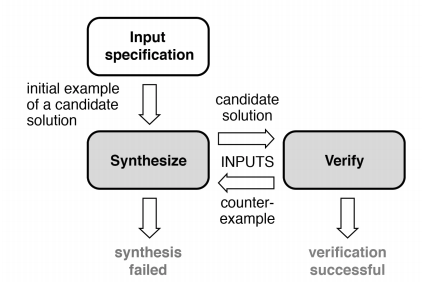
\includegraphics[width=0.75\columnwidth]{fig2_orig}
	\caption{Counterexample Guided Inductive Synthesis (CEGIS).}
	\label{Counter-Example-Guided-Inductive-Synthesis}
\end{figure}

The correctness specification $\sigma$ provided to our program synthesizer is of the form $\exists \vec{F} .  \forall \vec{x}.  \sigma(\vec{x}, \vec{F})$, where $\vec{F}$ ranges over functions, $\vec{x}$ ranges over ground terms, and $\sigma$ is a quantifier-free (QF) formula typically supported by SMT solvers. The ground terms are interpreted over some finite domain $\mathcal{D}$, where $\mathcal{D}$ can be encoded using the SMT's bit-vectors part. 

In Figure~\ref{Counter-Example-Guided-Inductive-Synthesis}, the  CEGIS method's {\sc Synthesize} and {\sc Verify} phases interact via a finite set of test vector {\sc inputs}, which is incrementally updated. Given the correctness specification $\sigma$, the {\sc Synthesize} procedure tries to find an existential witness $\vec{F}$ satisfying the specification $\sigma(\vec{x}, \vec{F})$, for all $\vec{x}$ in {\sc inputs} (as opposed to all $\vec{x} \in \mathcal{D}$). If {\sc Synthesize} succeeds in finding a witness~$\vec{F}$, the latter is a candidate solution (i.e., a feasible combination of equipment) for the full synthesis formula, which is passed to {\sc Verify} in order to check whether it is a proper solution ({\it i.e.}, $\vec{F}$ satisfies the specification $\sigma(\vec{x}, \vec{F})$ for all $\vec{x}\in\mathcal{D}$). If this is the case, then the algorithm terminates, i.e., we have found a feasible solution; otherwise, in the CEGIS method, additional information is provided for the {\sc Synthesize} phase, in the form of a new counterexample that is added to the {\sc inputs} set and the loop iterates again.

One may notice that each iteration of the CEGIS loop adds a new input to the finite set $\text{\sc inputs}$, which is then used for synthesis.  Given that the full set of inputs $\mathcal{D}$ is finite because we use bit-vector expressions, this means that the refinement loop can only iterate over a finite number of times. However, {\sc Synthesize} may conclude that no candidate solution obeying $\sigma$ for the finite set $\text{\sc inputs}$ exists and our synthesis engine can then conclude that no feasible solution was found.

\section{Solar Photovoltaic Systems}

According to \cite{Roy}, a PV system is designed to supply electrical loads. These loads can be of the Alternating Current (AC) type or the Direct Current (DC) type. The electricity supply can be needed either in daytime or nighttime (most cases, in both). The most basic PV system can supply only in daytime.  For the night hours or rainy days, batteries are needed, where power can be stored for later use~\cite{Gules}. 

PV systems are broadly classified into three distinct types, as described by \cite{Mohanty}: 

\begin{itemize}
\item Stand-alone systems, or off-grid systems, where the energy is generated and consumed in the same place and which does not interact with the main grid. Usually, the electricity consuming/utilizing device is part of the system, i.e., solar home systems, solar street lighting systems, solar lanterns, and solar power plants; 
\item Grid-connected systems, where the solar PV system is connected to the grid. The grid-connected system can be: 
\begin{itemize}
\item Grid-tied system, which can only feed power into the grid, with the result that this system cannot deliver power locally during blackouts and emergencies since these systems have to be completely disconnected from the grid and have to be shut down as per national and international electrical safety standards;
\item Some grid-connected PV systems, with energy storage, can also provide power locally in an islanding mode. 
\end{itemize}
\item Solar PV hybrid systems. In a hybrid system, other source(s) of energy, such as wind, biomass or diesel, can work together with the solar PV system to provide the required demand. In this type of system, the main objective is to bring more reliability into the overall system at an affordable cost by adding distinct energy sources.
\end{itemize}
 
In the specific case of isolated communities, depending on the type of load, cost, resources availability, and the load requirements, stand-alone systems can be split into several categories, as described below. Since the goal of this thesis is to present solutions only to isolated/ off-grid applications, on-grid or hybrid configurations are not discussed here.

\subsection{MPPT} 

There is a feature, called maximum power point tracking (MPPT), which is a control mechanism that maintains the PV panel operating at a voltage that corresponds to maximum power voltage, which maximizes the transfer of power while avoiding loss of PV cells \cite{Pinho}. This resource is found in modern PV systems and is strongly indicated due to its advantages.

\subsection{Unregulated Stand-alone PV Systems With DC Load }

Usually this type of system is for low power applications, as defined by \cite{Roy}. The PV system is directly connected to the load without any MPPT controller, as shown in Fig.\ref{fig:unregSPV}. At night, the system will not provide any power because of the absence of a battery. 
 
\begin{figure}[h]
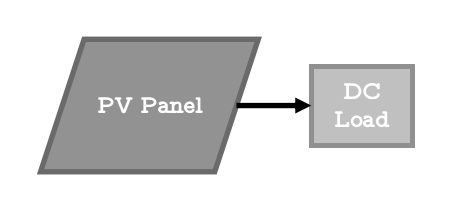
\includegraphics[width=0.6\textwidth]{unregulatedSPV.png}
\centering
\caption{Unregulated stand-alone solar PV system with DC load. Source: \cite{Roy}.}
\label{fig:unregSPV}
\end{figure}

\subsection{Regulated Stand-alone PV Systems With DC Load}
Similar to the unregulated stand-alone system with DC load, the main difference between this and the previous one is that this system requires a MPPT technique, as illustrated in Fig.\ref{fig:regSPV1}. Usually systems with MPPT should have a battery; otherwise, the extra power will be wasted. This is an inadequate use of PV systems, but it can be found in isolated communities in Brazil.

\begin{figure}[h]
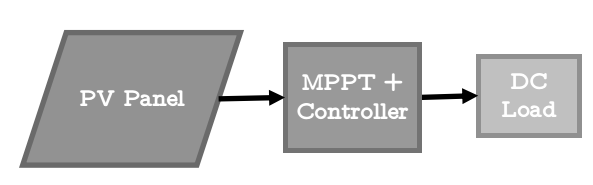
\includegraphics[width=0.8\textwidth]{regulatedSPV1.png}
\centering
\caption{Regulated stand-alone solar PV system with DC load. Source: \cite{Roy}.}
\label{fig:regSPV1}
\end{figure}

%%%%%%%%%%%%%%%%%%%%%%%%%%%%%%%%%%%%%%%%%%%%%%%%%%%%%%%%
\subsection{Regulated Stand-alone Systems With Battery and DC load}
%%%%%%%%%%%%%%%%%%%%%%%%%%%%%%%%%%%%%%%%%%%%%%%%%%%%%%%%

This configuration have PV array, battery, MPPT and DC load, as shown in Fig.\ref{fig:regSPV2}. The battery is used to store the extra power from the PV system. A charge controller is necessary for this type of system because it insures that the battery is charged with the correct voltage and current. Extra charging and deep discharging can reduce the battery life \cite{Kim}. The controller includes a DC-DC converter that is not shown in Fig.\ref{fig:regSPV2}, but it is inherent of a typical MPPT controller.

\begin{figure}[h]
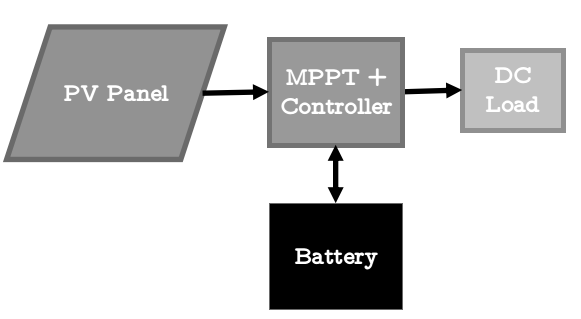
\includegraphics[width=0.8\textwidth]{regulatedSPV2.png}
\centering
\caption{Regulated stand-alone solar PV system with battery and DC load. Source: \cite{Roy}.}
\label{fig:regSPV2}
\end{figure}

A PV systems that are used to feed loads with low variation of consumption can be sized to operate without the controller. This is known as a self-regulated stand-alone PV system with battery. However, the PV panel voltage must be compatible with the battery voltage. Usually, the bank of batteries is oversized in relation to the PV panel and to the load. The drawback is the operation of the batteries, usually overloaded or with excessive discharges (that can damage the batteries).

%%%%%%%%%%%%%%%%%%%%%%%%%%%%%%%%%%%%%%%%%%%%%%%%%%%%%%%%
\subsection{Regulated Stand-alone Systems With Battery and AC load}
%%%%%%%%%%%%%%%%%%%%%%%%%%%%%%%%%%%%%%%%%%%%%%%%%%%%%%%%

This system is similar to the previous one, but the AC load draws the power from the PV system and, because of the AC load, an inverter (DC to AC converter) is required, as seen in Fig.\ref{fig:regSPV3}. This solution has a cost increase because it has more equipment. However, AC availability has the advantage of allowing the use of a higher number of AC appliances in homes or consumer units. This is the base configuration for this thesis since it is currently the most common system used specifically for remote rural areas of developing countries or areas where the grid extension is not feasible.
%stand-alone systems are one the most used solutions, and 
% depending on the type of load, cost, resources availability, and requirements of the load, 
%stand-alone systems 
%can be split into several categories. However, 
%the most suitable configuration is the regulated stand-alone system with battery and AC load.

\begin{figure}[h]
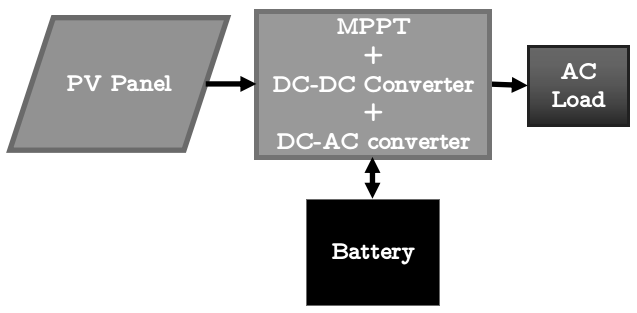
\includegraphics[width=0.8\textwidth]{regulatedSPV3.png}
\centering
\caption{Regulated stand-alone PV system with battery, AC load. Source: \cite{Roy}.}
\label{fig:regSPV3}
\end{figure}

%%%%%%%%%%%%%%%%%%%%%%%%%%%%%%%%%%%%%%%%%%%%%%%%%%%%%%%%
\subsection{Design and Validation of a Solar PV System}
%%%%%%%%%%%%%%%%%%%%%%%%%%%%%%%%%%%%%%%%%%%%%%%%%%%%%%%%

The design and validation of a solar PV system can be done by hand or with the aid of a software tool. 

In order to address different aspects of a project system and system's design, many commercial tools are available for the solar PV market. According to \cite{Brooks}, the capabilities of these tools range from simple solar resource and energy production estimation to site survey and system design tools, to sophisticated financial analysis software (with optimization). Some tools also provide support to rebate program applications and tax incentives (specific to each country or region). In contrast, other programs and worksheets focus on the technical aspects of system sizing and design.
 
Manufacturers and integrators also have their proprietary software to perform inverter string sizing and various system sizing and design tools, with the drawback of just including their products among the possibilities of choice. In this study, the most widely used tools are presented: 

\begin{itemize}
\item PVWatts 
\item SAM
\item Homer
\item RETScreen
\item Hybrid2
\end{itemize}

%%%%%%%%%%%%%%%%%%%%%%%%%%%%%%%%%%%%%%%%%%%%%%%%%%%%%%%%
\subsubsection{PVWatts Calculator}
%%%%%%%%%%%%%%%%%%%%%%%%%%%%%%%%%%%%%%%%%%%%%%%%%%%%%%%%

According to \cite{Freeman} and \cite{NRELDobos}, this is a web application developed by the National Renewable Energy Laboratory (NREL), which estimates the electricity production of a grid-connected roof- or ground-mounted photovoltaic system based on a few inputs. According to \cite{NRELDobos}, using the calculator requires information about the system's location, basic design parameters, and system economics. PVWatts calculates estimated values for the system's annual and monthly electricity production, and for the electricity's monetary value. This tool is suitable for very preliminary studies of a potential location for a photovoltaic system that uses crystalline silicon or thin-film photovoltaic modules. The production estimates that PVWatts computation does not account for many factors that are important in the design of a photovoltaic system, which makes it necessary to have the support of an energy expert. The calculator estimates the monthly and annual electricity production of a photovoltaic system using an hour-by-hour simulation over one year. To represent the system's physical characteristics, PVWatts requires values for six inputs: system DC size, module type, array type, system losses, array tilt angle, and array azimuth angle.

%%%%%%%%%%%%%%%%%%%%%%%%%%%%%%%%%%%%%%%%%%%%%%%%%%%%%%%%
\subsubsection{SAM}
%%%%%%%%%%%%%%%%%%%%%%%%%%%%%%%%%%%%%%%%%%%%%%%%%%%%%%%%

SAM or System Advisor Model is a software solution produced by the U.S. Department of Energy and National Renewable Energy Laboratory. According to \cite{NRELBlair} and \cite{Cameron2008}, SAM is intended to help users to determine whether the model meets their project constraints/specifications. SAM is a performance and financial model designed to facilitate decision making for people involved in the renewable energy industry: project managers and engineers; financial and policy analysts; technology developers; and researchers. SAM makes performance predictions and energy cost estimates for grid-connected power projects based on installation and operating costs and system design parameters that the user specifies as inputs to the model. Projects can be either on the customer side of the utility meter, where they buy and sell electricity at retail rates or on the utility side of the meter, where they sell electricity at a price negotiated through a power purchase agreement. SAM is an electrical power generation model and assumes that the renewable energy system delivers power either to an electric grid or to a grid-connected building or facility to meet the electric load. It does not model thermal energy systems that meet a thermal process load. As mentioned in \cite{NRELBlair}, SAM does not model isolated or off-grid power systems and does not model systems with electricity storage batteries.

%%%%%%%%%%%%%%%%%%%%%%%%%%%%%%%%%%%%%%%%%%%%%%%%%%%%%%%%
\subsubsection{HOMER}
%%%%%%%%%%%%%%%%%%%%%%%%%%%%%%%%%%%%%%%%%%%%%%%%%%%%%%%%

As defined in \cite{HOMER}, this is a set of two tools: HOMER Legacy and HOMER Pro. HOMER is an acronym for Hybrid Optimization Model for Multiple Energy Resources. HOMER Legacy is the original HOMER software version created at the National Renewable Energy Laboratory (NREL). HOMER Legacy is a free computer model that simplifies the task of evaluating design options for both off-grid and grid-connected power systems for remote, stand-alone, and distributed generation applications. HOMER's optimization and sensitivity analysis algorithms allow the user to evaluate the economic and technical feasibility of a large number of technology options. Since 2016 Homer Legacy can be found at the HOMER web site, but it is only available for students and nonprofit organizations, as defined in \cite{HOMER}, and has no support available. For a short time, only the commercial version will remain.
 
The commercial version (paid), known as HOMER Pro, as defined in \cite{Swarnkar}, is a tool for optimizing the microgrid design in all sectors, from village power and island utilities to grid-connected campuses and military bases. HOMER Pro puts together three tools in one product: optimization, simulation, and sensitivity analysis. It provides the full rigor of historical simulation and optimization in a model that is intended to be easy to use and is adaptable to a wide variety of projects. For a village or community-scale power system, HOMER can model both the technical and economic factors involved in the project. For larger systems, HOMER can provide an overview that compares the cost and feasibility of different configurations. Historical simulation is essential for modeling variable resources, such as solar and wind power, and for combined heat and power applications, where the thermal load is variable. HOMER's sensitivity analysis helps determine the potential impact of uncertain factors such as fuel prices or wind speed on a given system. 

%%%%%%%%%%%%%%%%%%%%%%%%%%%%%%%%%%%%%%%%%%%%%%%%%%%%%%%%
\subsubsection{RETScreen}
%%%%%%%%%%%%%%%%%%%%%%%%%%%%%%%%%%%%%%%%%%%%%%%%%%%%%%%%

As mentioned in \cite{Pradhan}, RETScreen is a decision-support tool designed to help decision-makers and energy professionals to evaluate the financial viability of renewable energy, energy efficiency, and/or co-generation projects.

RETScreen models various types of renewable energy technologies (RETs), allowing for comparisons between technology options. The software can be used to evaluate benefits from both clean energy production from power generation projects and savings through energy efficiency projects, accounting for project costs, greenhouse gas emission reductions, and financial risk. The software is freely distributed (but with restrictions to save work or print), and had three different versions:

\begin{itemize}
\item RETScreen 4 (discontinued, requires Microsoft Excel to run); 
\item RETScreen Software Suite, which includes the RETScreen 4 and a Windows-based graphical software that allows project owners to verify the ongoing energy performance of their facilities (discontinued in 2013);
\item And the current (2016) RETScreen Expert, which allows users to evaluate energy investments over an entire project life-cycle (including benchmarking, feasibility, and performance analysis) in a fully integrated way, and within one software platform. This version is only Windows-based and has a complete paid version via an annual subscription way.
\end{itemize}

As described by \cite{Pradhan}, RETScreen performs a standard five-step analysis: setting and site conditions, energy model, cost analysis, emission analysis, financial analysis, sensitivity, and risk analysis. It is developed and maintained by the Government of Canada through the CanmetENERGY Varennes Research Centre of Natural Resources, in collaboration with NASA; Renewable Energy and Energy Efficiency Partnership (REEEP); United Nations Environment Programme (UNEP), and the Global Environment Facility (GEF). RETScreen is available in 36 languages; it is a multi-awarded tool and includes equipment databases for components manufactured and available worldwide.

%%%%%%%%%%%%%%%%%%%%%%%%%%%%%%%%%%%%%%%%%%%%%%%%%%%%%%%%
\subsubsection{Hybrid2}
%%%%%%%%%%%%%%%%%%%%%%%%%%%%%%%%%%%%%%%%%%%%%%%%%%%%%%%%

The Hybrid2 software package, as described in \cite{Mills}, is a user-friendly tool that executes detailed long-term performance and economic analysis on a wide variety of hybrid power systems. Hybrid2 is a probabilistic/time series computer model, using time series data for loads, wind speed, insolation, and temperature. The power system is designed or selected by the user to predict the hybrid power system performance. Variations in wind speed and in load within each time step are factored into the performance predictions. The code does not consider short-term system fluctuations caused by system dynamics or component transients. This program is not supported anymore and according to \cite{UMASS}, probably after the user performs the free download of the tool, it will not work on Windows platforms later than Windows XP, which is a limitation.

Table~\ref{table:softwares} summarizes the tools described in this thesis, where just Hybrid2 is mentioned, no technical support is available. Only HOMER, RETScreen, and Hybrid2 perform off-grid system or battery backup analysis; all the tools perform solar photovoltaic analysis. Only HOMER and RETScreen are complete, including economic analysis and even optimization-sensitive analysis. However, only the paid version of these software packages have all the features, and they run only on Windows-based operating systems.

\begin{table}[!t]
%% increase table row spacing, adjust to taste
\renewcommand{\arraystretch}{1.3}
% if using array.sty, it might be a good idea to tweak the value of
% \extrarowheight as needed to properly center the text within the cells
\caption{Comparative coverage of reference softwares}
\label{table:softwares}
\centering
%% Some packages, such as MDW tools, offer better commands for making tables
%% than the plain LaTeX2e tabular which is used here.
\begin{tabular}{c | c | c | c | c | c}
\hline
\hline
Characteristic  & \rotatebox{90}{PVWatts} & \rotatebox{90}{SAM} & \rotatebox{90}{HOMER} & \rotatebox{90}{RETScreen } & \rotatebox{90}{Hybrid2}\\
\hline
Support & X & X & X & X &  \\
Off-grid systems &   &   & X & X & X\\
Hybrid systems &  &  & X & X & X\\
Photovoltaics & X & X & X & X & X\\
Batteries &  &  & X &  & X\\
Main technical (T) or economical (E) & T & T & E & E & T \\
Optimization &  &  & X & X &  \\
Sensitive analysis &  &  & X & X & \\
\hline
\hline
\end{tabular}
\end{table}

%%%%%%%%%%%%%%%%%%%%%%%%%%%%%%%%%%%%%%%%%%%%%%%%%%%%%%%%
\subsubsection{Thesis Proposal x Reference Tools}
%%%%%%%%%%%%%%%%%%%%%%%%%%%%%%%%%%%%%%%%%%%%%%%%%%%%%%%%

Considering that the focus of this research is on off-grid solutions and supported tools, only HOMER remains for comparison. All tools need some parameters inherently from the manufacturer's catalog, so the project starts with the manufacturer's and integrator's tool to define the essential items of the project: panels, inverters, controllers, and batteries. The potential solution is then analyzed by another tool to validate or even optimize the solution. The challenge of this study, therefore, is to prove that it is possible to use automated verification to validate an off-grid PV solution.

%%%%%%%%%%%%%%%%%%%%%%%%%%%%%%%%%%%%%%%%%%%%%%%%%%%%%%%%
\subsection{Component Models for Stand-alone PV Systems}
\label{sec:model}
%%%%%%%%%%%%%%%%%%%%%%%%%%%%%%%%%%%%%%%%%%%%%%%%%%%%%%%%

The primary purpose of this section is to describe the models for the elements of a stand-alone PV system: the PV generator, battery, controller, inverter, and load. The modeling of the PV system is based on modular blocks, as illustrated in Fig.\ref{fig:blockdiagram}, from \cite{Hansen}. The modular structure facilitates the modeling of the other system structures and the replacement of elements such as a DC load instead of an AC load. 

\begin{figure}[h]
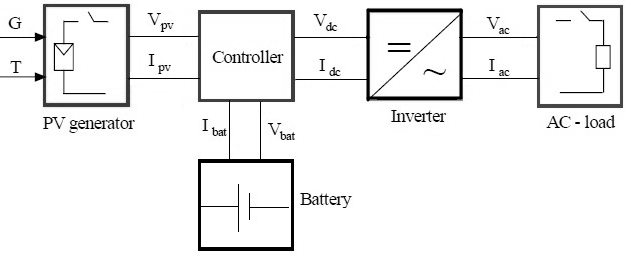
\includegraphics[width=0.95\textwidth]{blockdiagramPVS2}
\centering
\caption{Block diagram for the stand-alone PV system. Source: \cite{Hansen}.}
\label{fig:blockdiagram}
\end{figure}

In the literature, there are several mathematical models available for each component of stand-alone PV systems. In this section, the mathematical model for each component of PV system is presented. 

%%%%%%%%%%%%%%%%%%%%%%%%%%%%%%%%%%%%%%%%%%%%%%%%%%%%%%%%
\subsubsection{PV Generator (Cell, Module, String, and Array) }
%%%%%%%%%%%%%%%%%%%%%%%%%%%%%%%%%%%%%%%%%%%%%%%%%%%%%%%%

A photovoltaic PV generator is the whole assembly of solar cells, connections, protective parts, and supports. In the present modeling, the focus is only on the cell/module/array.
 
The fundamental element of a PV System is the PV cell, also called a Solar Cell. A PV / Solar Cell is a semiconductor device that can convert solar energy into DC electricity. The semiconductor materials (usually silicon), which are specially treated to form an electric field, positive on one side (backside) and negative on the other (towards the sun). When solar energy (photons) hits the solar cell, electrons are knocked loose from the atoms in the semiconductor material, creating electron-hole pairs \cite{Lorenzo}. If electrical conductors are attached to the positive and negative sides, forming an electrical circuit, the electrons are captured in the form of electric current $ I_{ph} $ (photocurrent).
 
In order to increase their application usage, many individual PV cells are interconnected together in a sealed, weatherproof package called Panel (or Module). For instance, a 12 V Panel will have 36 cells connected in series, and a 24 V Panel will have 72 PV cells connected in series. Besides, to achieve the desired voltage and current, modules are wired in series (strings) and parallel into what is called a PV array, as shown in Fig.\ref{fig:celmodarray}. The flexibility of the modular PV system allows designers to create PV systems that can meet a wide variety of electrical demands. 

\begin{figure}[h]
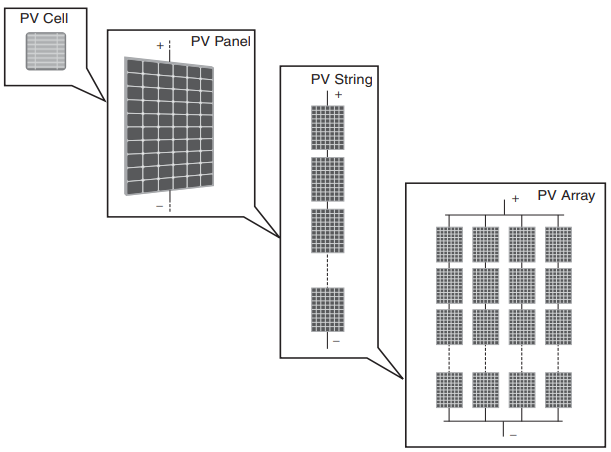
\includegraphics[width=0.95\textwidth]{PVarray}
\centering
\caption{PV cell, module, string and array. Source: \cite{SamlexSolar}.}
\label{fig:celmodarray}
\end{figure}

The PV modules are generally rated under standard test conditions (STC), which leads to the following specification by the manufacturers: solar radiation of 1000 W/m$^{2}$, cell temperature of 25$^{o}$C, and solar spectrum of 1.5. The parameters required for the input of the PV modules are dependent on the meteorological conditions of the area to be serviced by the photovoltaic solution. However, the climatic conditions are unpredictable due to the random nature of their occurrence \cite{Jakhrani}.
 
These uncertainties lead to either over- or underestimation of energy yield from PV modules. An overestimation of up to 40\% was reported as compared to the rated power output of PV modules \cite{Durisch}. 

The growing demand for photovoltaics technologies has led to research into the various aspects of its components from cell technology to the modeling, size optimization, and system performance \cite{Rajanna}, \cite{Badejani}; \cite{Yatimi}, \cite{Ferrari}, \cite{Saloux}, \cite{Hasan}, \cite{King}, \cite{Mellit}. Modeling PV modules is one of the major components responsible for the proper functioning of PV systems. However, the estimation of models is affected by various intrinsic and extrinsic factors, which ultimately influence the behavior of current and voltage. Therefore, the choice of the model is essential to estimate the performance of PV modules in different environmental conditions \cite{Jakhrani}.
 
Modeling provides the means to understand the current, voltage, and power relationships of PV systems.
  
The performance of photovoltaic systems (solar cells/panels), that is, the output current/voltage curve ($I-V$ curve), is usually studied using an equivalent circuit model. This equivalent circuit consists of a current source with one or two diodes connected in parallel, and up to two resistors, one connected in parallel and the other one in series, to take into account energy losses in this model \cite{Cubas}. Based on these electronic components, four basic configurations are usually used when studying PV systems, as shown in Fig. \ref{fig:equivckt}. 

\begin{figure}[h]
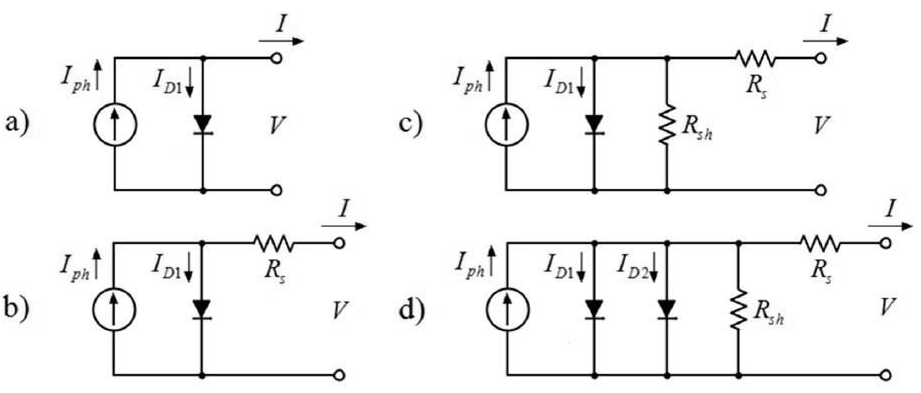
\includegraphics[width=0.95\textwidth]{equivckt}
\centering
\caption{Four different equivalent circuit models: (a) 1-diode; (b) 1-diode/1-resistor; (c) 1-diode/2-resistor; (d) 2-diode/2-resistor. Source: \cite{Cubas}.}
\label{fig:equivckt}
\end{figure}
 
The 1-diode model, whose equation to relate the output current, $I$, to the output voltage, $V$, is described in Equation \ref{eq:1diodemodel}. 

\begin{equation}
\label{eq:1diodemodel}
I = I_{ph}-I_{D1}=I_{ph}-I_{0}\left[ exp \left( \dfrac{V}{NaV_{T}} \right) -1 \right], 
\end{equation}

\noindent where:
\begin{itemize}
\item $I_{ph}$ is the photocurrent delivered by the constant current source. $I_{ph}$ is usually approximated to the reference short-circuit current of the PV panel ($I_{sc}$); 
\item $ I_{0} $ is the reverse saturation current corresponding to the diode; 
\item $ N $ is the number of series-connected cells in the photovoltaic system to be analyzed;
	\begin{itemize}
	\item $ N=1 $ in a single cell configuration. 	
	\end{itemize}	  
\item $ a $ is the ideality factor (or quality factor) that takes into account the deviation of the diodes from the Shockley diffusion theory; 
	\begin{itemize}
	\item $a=1$ for ideal diodes and between $ 1 $ and $ 2 $ for real diodes. 	
	\end{itemize}
\item $V_{T}$ is the thermal voltage ($ V_{T}=k_{B}T/q $);
	\begin{itemize}
	\item $ k_{B} $ is the Boltzmann constant ($ 1.3806503\times10^{-23}J/K $); 
	\item $ T $ is the temperature of the p-n junction (or cell temperature) expressed in Kelvin; 
	\item $ q $ is the absolute value of the electron's charge ($ -1.60217646\times10^{-19}C $).	
	\end{itemize}	 
\end{itemize}


This model has only three unknown parameters ($ I_{ph}$, $I_{0}$, and $a $), and it assumes that the series resistance is $ zero $ and shunt resistance is $ infinite $ and, thus, both of these parameters are ignored.
 
The 1-diode/1-resistor model, is described in Equation \ref{eq:1d1rmodel}. 

\begin{equation}
\label{eq:1d1rmodel}
I =I_{ph}-I_{0}\left[ exp \left( \dfrac{V+IR_{s}}{NaV_{T}} \right) -1 \right], 
\end{equation}

\noindent where $R_{s}$ is the series resistor.

In this model, there are four unknown parameters ($ I_{ph}$, $I_{0}$, $ R_{s} $, and $ a $), and it assumes shunt resistance as $ infinite $.

The 1-diode/2-resistor model, is described in Equation \ref{eq:1d2rmodel}. 

\begin{equation}
\label{eq:1d2rmodel}
I =I_{ph}-I_{0}\left[ exp \left( \dfrac{V+IR_{s}}{NaV_{T}} \right) -1 \right] - \dfrac{V+IR_{s}}{R_{sh}},
\end{equation}

\noindent where $R_{sh}$ is the shunt resistor.

In this model, there are five unknown parameters ($ I_{ph}$, $I_{0}$, $ R_{s} $, $ R_{sh} $, and $ a $).

And the 2-diode/2-resistor model, is described in Equation \ref{eq:2d2rmodel}. 

\begin{equation}
\label{eq:2d2rmodel}
I =I_{ph}-I_{01}\left[ exp \left( \dfrac{V+IR_{s}}{Na_{1}V_{T}} \right) -1 \right] - I_{02}\left[ exp \left( \dfrac{V+IR_{s}}{Na_{2}V_{T}} \right) -1 \right] - \dfrac{V+IR_{s}}{R_{sh}}
\end{equation}

This model has six unknown parameters with two exponential terms. 
Briefly, both single and double diode models require the knowledge of all unknown parameters, which is usually not provided by manufacturers. Nevertheless, the current-voltage equation is a transcendental expression \cite{Jakhrani}.  

However, regardless of the adopted model, the parameters of the equations must be estimated to adapt the corresponding model to the real behavior of the solar cell/panel. 

For this reason, researchers gradually focused on searching out the approximate methods for the calculation of unknown parameters, proceeding along three different paths. The analytical methods give exact solutions through algebraic equations, as done by \cite{Cubas} and \cite{Brano}. However, due to the inherent nature and nonlinearity of PV cell or module characteristics, it is hard to discover the analytical solution of all unknown parameters, as described in \cite{Hasan}. Thus, numerical methods such as the Newton-Raphson method or the Levenberg-Marquardt algorithm were preferred, as described by \cite{Mellit}. This happens because numerical methods give approximate solutions to nonlinear problems without searching for exact solutions. However, numerical methods are time-consuming and need long term time series data, which may not be available in developing countries. Reference~\cite{Jakhrani} used mixed methodology, bringing analytical and numerical steps together. \cite{Shenawy} et al. create a method to discover the unknown parameters of the PV panels through experimentation. Furthermore, \cite{Tian} used a mix of analytical and experimental methodology to establish the unknown parameters. However, samples of the PV modules are necessary to perform some tests when we use the experimental technique. 

Therefore, a wide variety of models exists for estimation of the power output of PV modules (and $I-V$ or $P-V$ curves). However, this study will rely on the simplified 1-diode model, which was shown by \cite{Saloux} that has a small error rate, between 0.03\% and 4.68\% for the selected PV panels tested. Besides, this mathematical modeling has the advantage of being an explicit model, which does not use iterative numerical calculation. 

%%%%%%%%%%%%%%%%%%%%%%%%%%%%%%%%%%%%%%%%%%%%%%%%%%%%%%%%
\subsubsection{The Proposed PV Panel Model}
%%%%%%%%%%%%%%%%%%%%%%%%%%%%%%%%%%%%%%%%%%%%%%%%%%%%%%%%

With the proposed model, an explicit set of equations is derived from the ideal PV model given by Equation~\ref{eq:1diodemodel}.

A single-diode without series and shunt resistances is considered. Equation~\ref{eq:1diodemodel} is used to write down expressions for currents and voltages at each key point shown in Fig. \ref{fig:ivcurve}. Note that the MPPT point from the PV panel is illustrated, highlighting the maximum voltage $ V_{m} $ and maximum current $ I_{m} $ that a panel can produce.

\begin{figure}[h]
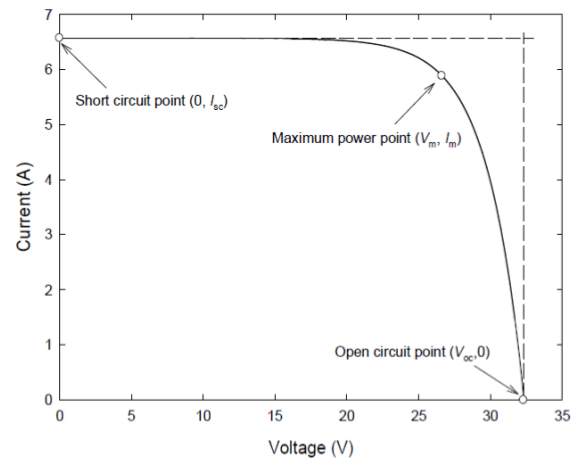
\includegraphics[width=0.7\textwidth]{ivcurve}
\centering
\caption{$ I-V $ characteristic curve of an ideal PV cell. Source: \cite{Saloux}.}
\label{fig:ivcurve}
\end{figure}

Hence, the short-circuit current, the open-circuit voltage, the maximum power voltage and current are written as defined by \cite{Saloux} and shown in Equations \ref{eq:Isc} to \ref{eq:Im}.

\begin{equation}
\label{eq:Isc}
I_{sc}=I_{ph}\vert_{V=0}
\end{equation}

\begin{equation}
\label{eq:Voc}
V_{oc}=\dfrac{aNk_{B}T}{q}ln\left( 1+\dfrac{I_{sc}}{I_{0}} \right) 
\end{equation}

\begin{equation}
\label{eq:exp}
exp\left( \dfrac{qV_{oc}}{aNk_{B}T} \right) = \left(1+\dfrac{qV_{m}}{aNk_{B}T} \right) exp \left( \dfrac{qV_{m}}{aNk_{B}T} \right) 
\end{equation}

\begin{equation}
\label{eq:Im}
I_{m} =I_{ph}-I_{0}\left[ exp \left( \dfrac{qV_{m}}{aNk_{B}T} \right) -1 \right] 
\end{equation}

Equations \ref{eq:exp} and \ref{eq:Im} are not explicit with regard to the key PV  parameters, it therefore needs to be rewritten in a different way. A PV cell has a hybrid behavior, i.e., a current-source at the short-circuit point and a voltage-source at the open-circuit point \cite{Saloux}. These two regions are characterized by two asymptotes of the $ I-V $ curve in Fig. \ref{fig:ivcurve}, where the transition is a compromise between both behaviors. It is interesting to observe that the maximum power point corresponds to a trade-off condition, where the current is still high enough before it starts decreasing with the increase in the output voltage (Fig. \ref{fig:ivcurve}).

Based on this, the tangent of the I-V curve can be used to evaluate the transition between current- to voltage-source controlled regions; this operation yields Equation \ref{eq:didv}.

\begin{equation}
\label{eq:didv}
\dfrac{dI}{dV}=-\dfrac{qI_{0}}{aNk_{B}T}exp \left( \dfrac{qV}{aNk_{B}T}  \right) 
\end{equation}

Equation \ref{eq:didv} is used to calculate the output voltage that corresponds to the maximum power operation condition of the cell, thus generating the Equation \ref{eq:Vmderiv}.

\begin{equation}
\label{eq:Vmderiv}
V_{m}=\dfrac{aNk_{B}T}{q} ln \left( -\dfrac{aNk_{B}T}{qI_{0}} \left( \dfrac{dI}{dV}  \right)_{V_{m}}   \right) 
\end{equation}

It is evident that Equation \ref{eq:Vmderiv} requires an expression of the derivative of the current with voltage evaluated at the maximum power point. The fact that the maximum power corresponds to an extreme, the variation of the maximum output power with voltage is relatively small, i.e., a change in $ V_{m} $ has a relatively small effect on the maximum power of the cell \cite{Saloux}. Consequently, considering the asymptotic behavior of the $I-V$ curve in short- and open-circuit conditions, the derivative required by Equation 10 can be calculated as shown in Equation \ref{eq:dIdV_Vm}.

\begin{equation}
\label{eq:dIdV_Vm}
\dfrac{dI}{dV}\vert_{V_{m}} \cong -\dfrac{0-I_{sc}}{V_{oc}-0}=\dfrac{I_{sc}}{V_{oc}}
\end{equation}

Replacing the Equation \ref{eq:dIdV_Vm} into Equations \ref{eq:Vmderiv} and \ref{eq:Im}, the voltage and the current at the maximum power point and consequently the maximum output power, are expressed by Equations \ref{eq:Vmfinal}, \ref{eq:Imfinal}, and \ref{eq:Pm} ($ P_{m}=V_{m}I_{m} $). These equations are used to calculate the key cell parameters at the maximum power point (MPPT) as a function of cell temperature and parameters from the manufacturer's data-sheet.

\begin{equation}
\label{eq:Vmfinal}
V_{m}=\dfrac{aNk_{B}T}{q} ln \left( \dfrac{aNk_{B}T}{qI_{0}} \dfrac{I_{sc}}{V_{oc}}  \right) 
\end{equation}

\begin{equation}
\label{eq:Imfinal}
I_{m} = I_{ph} + I_{0} - \dfrac{aNk_{B}T}{q} \left( \dfrac{I_{sc}}{V_{oc}} \right)  
\end{equation}

\begin{equation}
\label{eq:Pm}
P_{m} = \left[ \dfrac{aNk_{B}T}{q} ln \left( \dfrac{aNk_{B}T}{qI_{0}} \dfrac{I_{sc}}{V_{oc}}  \right) \right] \times \left[ I_{ph} + I_{0} - \dfrac{aNk_{B}T}{q} \left( \dfrac{I_{sc}}{V_{oc}} \right)  \right] 
\end{equation}


However, the photocurrent delivered by the constant current source ($ I_{ph} $) or even the reverse saturation current ($ I_{0} $) is not given by PV manufacturers. Therefore, Equation \ref{eq:Iph} is used to calculate the photocurrent as a function of irradiance and temperature \cite{Villalva}.

\begin{equation}
\label{eq:Iph}
I_{ph}=\dfrac{G}{G_{ref}} \left[ I_{ph,ref} + \mu_{I} \left( T-T_{ref} \right)    \right] 
\end{equation}

\noindent where the reference state (STC) of the cell is given by the solar irradiance $ G_{ref}=1000 W/m^{2} $, and the temperature $ T_{ref}=298.15 K (=25^{o}C) $.

In Equation \ref{eq:Iph}, $ \mu_{I} $ is the short-circuit current temperature coefficient ($A/K$) and corresponds to the photocurrent obtained from a given PV cell working at (STC or standard test conditions) reference conditions (provided by PV manufacturers). $ I_{ph,ref} $ can also be approximated to the reference short-circuit current that is provided by PV manufacturers ($ I_{sc,ref} $) as shown by \cite{Jakhrani}.

The cell temperature ($ T $) can be obtained from \cite{Ross} and is shown in Equation \ref{eq:Tcell}.

\begin{equation}
\label{eq:Tcell}
T = T_{air} + \dfrac{NOCT-20}{800}G
\end{equation}

\noindent where $ T_{air} $ is the ambient temperature, $NOCT$ is the nominal operating cell temperature (in $^{o}$C) that is found on the PV manufacturer's data-sheet, and $G$ is the solar irradiance ($ W/m^{2} $) at the location of the PV system. In this thesis is not considered shading, which can impact in the cell temperature as well.

Furthermore, \cite{Villalva} have proposed a relationship, which allows the saturation current ($ I_{0} $) to be expressed as a function of the cell temperature. In this study, this relation is explicitly written based on cell open-circuit conditions using the short-circuit current temperature coefficient in addition to the open-circuit voltage temperature coefficient (Equation \ref{eq:I0}).

\begin{equation}
\label{eq:I0}
I_{0} = \dfrac{I_{sc,ref} + \mu_{I}(T - T_{ref})}{exp \left[ \dfrac{q(V_{oc,ref} + \mu_{V} (T - T_{ref}))}{aNk_{B}T}    \right] -1}
\end{equation}

\noindent where $ V_{oc,ref} $ is the reference open-circuit voltage, and $ \mu_{V} $ is an open-circuit voltage temperature coefficient ($ V/K $).

The ideality (or quality) factor of the diode $ a $, which is usually considered as a constant \cite{Villalva}, is determined in the reference state. Using the maximum power point current equation (Equation \ref{eq:Pm}) and the saturation current in the reference temperature given by Equation \ref{eq:I0}, the diode quality coefficient is determined by Equation \ref{eq:a}.

\begin{equation}
\label{eq:a}
a = \dfrac{q(V_{m,ref}-V_{oc,ref})}{Nk_{B}T} \dfrac{1}{ln \left( 1 - \dfrac{I_{m,ref}}{I_{sc,ref}}  \right) }
\end{equation}

\noindent where $ V_{mref} $, $ V_{oc,ref} $, $ I_{m,ref} $, and $ I_{sc,ref} $ are key cell values obtained under both actual cell temperature and solar irradiance conditions, usually provided by the manufacturers.

The model is now completely determined, i.e., with all the variables defined. This model requires the actual cell temperature (or the air temperature), the actual solar irradiance and common data provided by manufacturers.

If the PV cells are in parallel, then there is a parallel array. There will therefore be a change in the $ I_{ph} $ and $ I_{0} $ and the resulting current is given by Equation \ref{eq:Iarray}, as demonstrated in \cite{Saloux}.

\begin{equation}
\label{eq:Iarray}
I_{array} = (N_{cells in parallel})(I_{one cell})
\end{equation}

\noindent where $ I_{one cell} $ is the current from Equation \ref{eq:Imfinal}.

In addition, if the panels are in series, the current does not change but the total voltage is the sum of the voltage of each individual panel.

\begin{equation}
\label{eq:Varray}
V_{array} = (N_{cells in series})(V_{one panel})
\end{equation}

\noindent where $ V_{one panel} $ is the maximum voltage from Equation \ref{eq:Vmfinal}.

%%%%%%%%%%%%%%%%%%%%%%%%%%%%%%%%%%%%%%%%%%%%%%%%%%%%%%%%
\subsubsection{Battery Storage Model}
%%%%%%%%%%%%%%%%%%%%%%%%%%%%%%%%%%%%%%%%%%%%%%%%%%%%%%%%

Because of the fluctuating nature of the output delivered by the PV arrays, batteries are an essential part of a PV system. Thus, during the hours of sunshine, the PV system feeds the load directly and excess electrical energy is stored in the batteries. During the night, or during a period with low solar irradiation, energy is supplied to the load from the battery bank ~\cite{Mellit}.
  
Several models have been presented in the literature. However, regardless of the model, the following parameters are usually required\cite{Mellit}: 

\begin{itemize}
\item Nominal capacity ($ q_{m} $), is the number of Ampere-hours ($ Ah $) that can maximally be extracted from the battery, under predetermined discharge conditions.
\item State of charge ($ SOC $), is the ratio between the present capacity and the nominal capacity, i.e., $ SOC = q/q_{max} $. Obviously $ 0<SOC<1 $. If $ SOC=1 $, then the battery is totally charged; and if $ SOC=0 $, the battery is fully discharged.
\item Charge (or discharge) regime. This parameter reflects the relationship between the nominal capacity of a battery and the current at which it is charged (or discharged). It is expressed in hours. %: for instance, discharge regime is 30h for a battery of 150 Ah that is discharged at 5A.
\item Efficiency ($\eta_{b}$), is the ratio of the charge extracted during discharge divided by the amount of the charge needed to restore the initial state of charging or discharging current. 
\item Lifetime, is the number of charge/discharge cycles the battery can sustain before losing 20\% of its nominal capacity.
\end{itemize}

The merit of a stand-alone PV system is evaluated in terms of the reliability of the electricity supply to the load and in terms of the long-term efficiency of the components. Battery efficiency was described in this section, and the reliability is quantified by the concept of loss of load probability (LLP). LLP is defined as the ratio between the Ampere-hour deficit and the Ampere-hour demand, both with respect to the load, over a long period of time \cite{Copetti}. 

In general, the battery models view the battery as a voltage source $ E $ in series with an internal resistance $ R_{0} $, as shown in Fig. \ref{fig:batteryckt}. 

\begin{figure}[h]
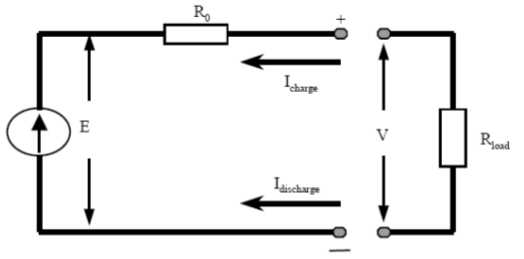
\includegraphics[width=0.5\textwidth]{batteryckt}
\centering
\caption{Schematic diagram of the battery. Source: \cite{Hansen}.}
\label{fig:batteryckt}
\end{figure}

%The terminal voltage of the battery can be expressed in terms of its open circuit voltage and the voltage across the internal resistance of the battery \cite{Sukamongkol}, as shown by Equation 31.  
%Where $ V_{b} $ is the battery terminal voltage, $ E_{oc} $ is the battery circuit voltage, $ I_{b} $ is the battery current, and $ R_{b} $ is the internal resistance of the battery.

The battery model, which describes the relationship between the voltage, the current and the state of charge, can be found in \cite{Copetti}, \cite{Manwell93}, and \cite{Manwell94}.  

Manwell and McGowen's Kinetic Battery Model (KiBaM)  \cite{Manwell93} was developed at the University of Massachusetts to predict the performance of the battery, based on manufacturer's data. However, it uses some data extracted from batteries tested in laboratory. It is therefore not suitable for this study. 

Most of the models created were used to simulate and optimize PV storage systems based on lead-acid batteries, the most commonly used batteries in developing countries, owing to their relative low cost and wide availability. % \cite{Copetti}. 
Batteries with modern technologies, as nickel–cadmium battery (NiCd), nickel metal hydrate (NiMH), lithium-ion (Li-ion), among others, although they have advantages (greater efficiency, longer life-time, greater depth of discharge), they are generally not economically viable in most PV systems. Table~\ref{table:batteries} shows the main features of some rechargeable batteries that are available at the market nowadays.

\begin{table}[!t]
%% increase table row spacing, adjust to taste
\renewcommand{\arraystretch}{1.3}
\caption{Technical data for some rechargeable batteries. Adapted from \cite{Pinho}}
\label{table:batteries}
\centering
\begin{tabular}{c | c | c | c | c }
\hline
\hline
Technology & \makecell{Efficiency \\ \%} & \makecell{Life Time \\ years} & \makecell{Number of \\ Cycles} & \makecell{Operational \\ Temperature}\\
\hline
Lead-acid (Pb-acid) & 80-90 & 3-20 & 250-500 & -15 to +50 \\
\hline
Nickel–cadmium (NiCd) & 60-70 & 3-25 & 300-700 & -45 to +50 \\
\hline
Nickel metal hydrate (NiMH) & 80-90 & 2-5 & 300-600 & -20 to +60 \\
\hline
Lithium-ion (Li-ion) & 90-95 & - & 500-1000 & -20 to +60 \\
\hline
\hline
\end{tabular}
\end{table}

Here, the model adopted is the based on \cite{Copetti}, who uses manufacturer's data and allows finding relations among voltage, current, state of charge and temperature. 

The discharge voltage equation is shown in Equation \ref{eq:bat_Vd}. The first term represents the voltage variation with the state of charge ($ SOC $), i.e., the electrolyte concentration, and the second is the variation due to internal resistance variation.

\begin{equation}
\label{eq:bat_Vd}
V_{d} = \left[ 2.085-0.12(1-SOC) \right] - \dfrac{I}{C_{10}} \left( \dfrac{4}{1+I^{1.3}} + \dfrac{0.27}{SOC^{1.5}}+0.02 \right) (1-0.007 \Delta T)
\end{equation}

\noindent where $ C_{10} $ means 10h of rated capacity, which is standard on the manufacturer's data-sheet, $ \Delta T $ is temperature variation ($ \Delta T=T-T_{ref} $, $ T_{ref}=25^{o}C $, $ SOC $ indicates how much electric charge is stored in the cell at any given time, defined by Equation \ref{eq:SOCbat}.

\begin{equation}
\label{eq:SOCbat}
SOC = \left( 1 - \dfrac{Q}{C} \right) 
\end{equation}

\noindent where $ Q $ is the charge delivered at the time of interest ($ Q=It $), and C is the battery capacity.

The ratio between $ Q $ and $ C $ represents the depth of discharge ($ DOD $) or the fraction of discharge, i.e., $ DOD=1-SOC $.
However it is worth to separate the $DOD$ into two different definitions when the battery autonomy is bigger than one day ($24$ hours). Therefore, here in this thesis, the definition given here is for maximum $DOD$. When we deal with daily $DOD$ we will call it of $DOD_{day}$, and obviously the sum of every $DOD_{day}$ can not exceed the maximum $DOD$.

The efficiency of the battery discharge is assumed to be 100\%, according to \cite{Copetti}; however, the total amount of useful charge available during discharge is limited by the current rate and temperature given by Equation \ref{eq:CC10}. This equation, known as capacity, is normalized with respect to discharge current corresponding to $ C_{10} $ rated capacity ($ I_{10} $).

\begin{equation}
\label{eq:CC10}
\dfrac{C}{C_{10}} = \dfrac{1.67}{1+0.67 \left( \dfrac{I}{I_{10}} \right)^{0.9} }(1+0.005 \Delta T)
\end{equation}

Note that when the discharge current tends to zero at 25$^{o}$C, the maximum capacity that can be removed is about 67\% over the $C_{10}$ capacity.

For the charging process, however, the parameters are presented in Equation \ref{eq:Vcbat}.

\begin{equation}
\label{eq:Vcbat}
V_{c} = [2+0.16SOC]+ \dfrac{I}{C_{10}} \left( \dfrac{6}{1+I^{0.86}} + \dfrac{0.48}{(1-SOC)^{1.2}} + 0.036  \right) (1-0.025 \Delta T)
\end{equation}

SOC can be calculated easily at any point during the discharge period; however, during recharge it is much more difficult \cite{Copetti}.

Generally, the efficient region is where $ SOC $ is below $ 0.7 $ and $ V_{c} $ is less than $2.3 V$ per cell. The efficiency drops to zero at full charge and the function that represents the charge efficiency ($ \eta_{c} $) variation with state of charge and current rate is given in Equation \ref{eq:efficcharge}.

\begin{equation}
\label{eq:efficcharge}
\eta_{c} = 1 - exp \left[ \dfrac{20.73}{\dfrac{I}{I_{10}}+0.55} (SOC-1) \right] 
\end{equation}

\cite{Copetti} show that, during overcharge, gassing occurs and tests have demonstrated that the final charge voltage ($ V_{ec} $) increases with the current intensity and with the decrease in temperature (Equation \ref{eq:Vec}). A function was created for the gassing voltage also, as shown in Equation \ref{eq:Vg}. In addition, the overcharge phenomenon can be represented by Equation \ref{eq:Voverc}.

\begin{equation}
\label{eq:Vec}
V_{ec} = \left[ 2.45 + 2.011 ln \left( 1+\dfrac{I}{C_{10}} \right)  \right] (1-0.002 \Delta T)
\end{equation}

\begin{equation}
\label{eq:Vg}
V_{g} = \left[ 2.24 + 1.97 ln \left( 1+\dfrac{I}{C_{10}} \right)  \right] (1-0.002 \Delta T)
\end{equation}

\begin{equation}
\label{eq:Voverc}
V_{c} = V_{g} + (V_{ec} - V_{g}) \left[ 1- exp \left( \dfrac{Ah_{restored}-0.95C}{I\tau}  \right)    \right] 
\end{equation}

\noindent where $ Ah_{restored} $ represents the Ampere-hour stored in the battery with regard to the battery capacity ($ C $) during this hour.

The function assumes that 95\% of the capacity has already been restored at the start of overcharge.

The time constant of the phenomenon ($ \tau $) is inversely proportional to the charge intensity and can be written as Equation \ref{eq:tau}.

\begin{equation}
\label{eq:tau}
\tau = \dfrac{17.3}{1+852 \left( \dfrac{I}{C_{10}} \right) ^{1.67} }
\end{equation}

Equation \ref{eq:Vcbat} can therefore be used to model the voltage ($ V_{c} $) evolution of the battery, at the start of gassing ($ V_{c} \leq V_{g} $). During overcharging ($ V_{c} > V_{g} $), Equation \ref{eq:Voverc} can be used until a constant final voltage ($ V_{ec} $) is reached.

The battery's storage capacity can be calculated using Equation \ref{eq:stor}, as defined in \cite{Wenham}.

\begin{equation}
\label{eq:stor}
Storage \, capacity = \dfrac{N_{C}E_{load}}{DOD \eta _{b}}
\end{equation}

\noindent where $ DOD $ is the maximum possible depth of battery discharge, $ E_{load} $ is the average energy consumed by the load corrected according PV equipment efficiency, $ N_{C} $ is the largest number of continuous cloudy days of the area, and $ \eta_{b} $ is the efficiency of the battery.

As an example of this formula's application, as shown in \cite{Abdulateef}, considering that an off-grid PV system is intended to supply $1.5 kW/48 V$ for 24 hours ($=36 kWh$); The largest number of continuous cloudy days in the selected site is about 1 day; For a maximum depth of battery discharge $DOD$ of $0.8$ and battery efficiency at $80\%$. 

In this thesis, the adopted efficiency of the battery will be considered constant and equal to $86\%$ as expected to lead-acid batteries~\cite{Pinho}.

Using Equation \ref{eq:stor}, the storage capacity then becomes $56.3 kWh$. Since the selected DC bus voltage is $48 V$, then the required Ampere-hours of the battery is $1173 Ah$ ($56.3 kWh/48$). If a single battery is 12 V and 350 Ah, then four batteries are connected in series ($4 \times 350 Ah = 1400 Ah$) and a total of 16 batteries is defined (an array of 4 to reach the 48 V of the DC bus in four arrays to feed the $Ah$ demanded).

In this study, a simplified model for battery charging (Equation \ref{eq:charge}) and discharging (Equation \ref{eq:discharge}) was considered, even recognizing that the process is not linear and is temperature-dependent. The equations are used to update the $SOC$ of the batteries, and have the number of hours ($ Num_{h} $) as a variable. There is a factor (1.15) which is present in the charging equation, and is necessary to express that during the charging process it is usual to reach 115\% of the battery capacity.

\begin{equation}
\label{eq:charge}
SOC_{charge} = SOC_{previous} + \dfrac{100*Pm*Num_{h}}{V_{system}*capacity*N_{BP}*1.15}
\end{equation}

\begin{equation}
\label{eq:discharge}
SOC_{discharge} = SOC_{previous} - \dfrac{100*I_{drained}*Num_{h}}{capacity}
\end{equation}

It is worth mentioning that, specifically for PV systems used in Brazil, a Regulation (RN 493/2012), issued by the Brazilian Electricity Regulatory Agency (ANEEL) recommends a minimum of 48 hours of battery autonomy for stand-alone solar PV systems, among others related definitions.

%%%%%%%%%%%%%%%%%%%%%%%%%%%%%%%%%%%%%%%%%%%%%%%%%%%%%%%%
\subsubsection{Controller Model}
\label{sec:controller}
%%%%%%%%%%%%%%%%%%%%%%%%%%%%%%%%%%%%%%%%%%%%%%%%%%%%%%%%

The controller is named differently by different authors: controller \cite{Hansen}, charge controller \cite{Mahanta} and \cite{Chauhan}, regulator \cite{Mellit}, DC-DC converter with MPPT and switch \cite{Dhanowa}, \cite{Yatimi}, \cite{Abdulateef}, \cite{Roy}. However, in this study, in order to simplify, the term used is controller. 

The controller is a set of items (DC-DC converter, a MPPT algorithm and switches) and can be defined as the responsible for managing the energy flow to the PV system, batteries and loads by collecting information on the battery voltage and knowing the maximum and minimum values acceptable for the battery voltage. Controllers aim to protect the battery (or batteries) against the excessive charge and discharge, improving its lifetime. 

Currently, controllers with MPPT algorithms are the most widely used nowadays,  and they maintain the PV operating at the stage of maximum power.

As defined by \cite{Hansen} and \cite{Mellit}, all power systems must include a control strategy, which describes the interactions between its components. The use of a battery as a storage form thus implies the presence of a charge controller. 

In general, there are two main operating modes for the controller: normal operating condition, when the battery voltage fluctuates between maximum and minimum voltages; and overcharge or over-discharge conditions, which occur when the battery voltage reaches some critical values. 

\cite{Mellit} established that the controller allows the management of energy between the load and the battery. The input signals for the regulator model are the battery current, the PV generator's voltage, the PV generator's current, and battery voltage. The outputs are battery current and used current. 

According to \cite{Hansen}, in order to protect the battery against an excessive charge, the PV arrays are disconnected from the system, whenever the terminal voltage increases above a certain threshold $ V_{max \textunderscore off} $ and whenever the current required by the load is less than the current delivered by the PV arrays. PV arrays are connected again when the terminal voltage decreases below a certain value $ V_{max \textunderscore on} $. This can be done by using a switch with a hysteresis cycle, as illustrated in Fig. \ref{fig:controllerover} in a on-off charge controller model.

\begin{figure}[h]
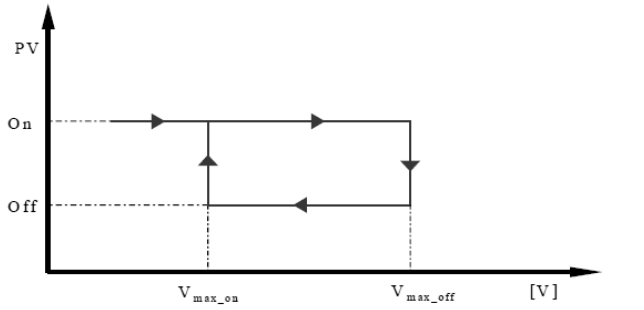
\includegraphics[width=0.7\textwidth]{controllerover}
\centering
\caption{Operating principle of an overcharge protector. Source: \cite{Hansen}.}
\label{fig:controllerover}
\end{figure}

To protect the battery against excessive discharge, the load is disconnected whenever the terminal voltage falls below a certain threshold $i$ and when the current required by the load is larger than the current delivered by the PV arrays \cite{Hansen}. The load is reconnected to the system, when the terminal voltage is above a certain value $i$, using a switch with a hysteresis cycle, as shown in Fig. \ref{fig:controllerdisc}. 

\begin{figure}[h]
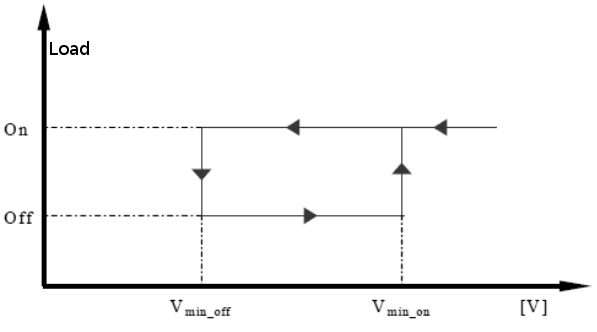
\includegraphics[width=0.7\textwidth]{controllerdisc}
\centering
\caption{Operating principle of a discharge protector. Source: \cite{Hansen}.}
\label{fig:controllerdisc}
\end{figure}

According to \cite{Lorenzo}, the switches may either be electromechanical (relay, contactors, etc.) or solid state (bipolar transistors, MOSFET's, etc.). 

The steps in the modeling of the controller process are summarized in Table \ref{table:controller}.

\begin{table}[!t]
%% increase table row spacing, adjust to taste
\renewcommand{\arraystretch}{1.3}
% if using array.sty, it might be a good idea to tweak the value of
% \extrarowheight as needed to properly center the text within the cells
\caption{Summary of the controller process. Source: adapted from~\cite{Hansen}}
\label{table:controller}
\centering
%% Some packages, such as MDW tools, offer better commands for making tables
%% than the plain LaTeX2e tabular which is used here.
\begin{tabular}{c | c | c }
\hline
\hline
Step  & Constraint & Command\\
\hline
\hline
(1) & \makecell{If $V > V_{max \_ off}$ \\and $I_{load} < I_{pv}$} & \makecell{Disconnect PV array \\from the system}\\
\hline
(2) & \makecell{If command (1) is \\done and $V < V_{max \_ on}$} & \makecell{Reconnect PV array \\to the system}\\
\hline
(3) & \makecell{If $V < V_{min \_ off}$ and \\ $I_{load} > I_{pv}$} & \makecell{Disconnect the load \\from the system}\\
\hline
(4) & \makecell{If command (3) is \\ done and $V > V_{min \_ on}$} & \makecell{Reconnect the load \\to the system}\\
\hline
\hline
\end{tabular}
\end{table}

As to the DC-DC converter, the most basic idea is that the power is converted while altering the current and voltage. 

As shown in \cite{Abdulateef}, the DC-DC converter is used to increase the efficiency of the PV system by matching the voltage generated by the PV array to the voltage required by the load. The output power ($ P_{out} $) of the DC-DC converter is given by Equation \ref{eq:poutcont}. 

\begin{equation}
\label{eq:poutcont}
P_{in} \eta_{c} = P_{out}
\end{equation}

Assuming that the efficiency of the controller ($ \eta_{c} $) is data provided by the manufacturer (ideally constant in this thesis), from Equation \ref{eq:poutcont} it is possible to reach Equation \ref{eq:potcont}.

\begin{equation}
\label{eq:potcont}
V_{in} I_{in} \eta_{c} = V_{out} I_{out}
\end{equation}

\noindent where $ V_{in} $ is the voltage across the PV array, $ I_{in} $ is the current output of the PV array, $ V_{out}$ is the  DC bus voltage, and $I_{out}$ is the output current from the converter, when all the other values are known.

It is worth mentioning that, depending on the PV panel generation and on the batteries charge, $ V_{out}$ can be the voltage that charges the battery $V_{b}$ (which is greater than the nominal voltage of the batteries), the voltage that is feed by the batteries (the same $V_{b}$ but with levels that can be lower), or even the voltage that comes from the PV panels and depends on the MPPT system employed by the controller.

The output voltage is related to the input voltage as a function of the duty cycle of the switch (\cite{Abdulateef}). 
 
A DC-DC converter used in these applications can either be step-up (Boost), step-down (Buck), or both increase and decrease (Buck-Boost) the voltage, as defined by \cite{Mahanta}. In addition, there is the Cúk converter, which is a Buck-Boost converter with an inverting topology \cite{Catherine}. 

For the Cúk converter, the relationship is expressed by Equation \ref{eq:voutvin} as shown in \cite{Abdulateef}.

\begin{equation}
\label{eq:voutvin}
\dfrac{V_{out}}{V_{in}} = \dfrac{D}{D-1}
\end{equation}

\noindent where $D$ is the duty cycle or ratio of the circuit converter, i.e., it is defined as the ratio of the on time of the switch to the total switching period.
 
The DC/DC converter tries always to operate in the MPPT to maximize the PV array efficiency and consequently increase the efficiency of the PV system, as defined in \cite{Yatimi}.
  
Various types of MPPT schemes are proposed by researchers, namely open circuit, short circuit, perturb and observe (P\& O)/hill climbing, incremental conductance, and so forth, as shown in  \cite{Haque}.
 
As the MPPT definition and the equations to get the maximum power from the PV panels were described at the end of the PV panel modeling, what is important here is that Equation \ref{eq:potcont} defines the relationship between the input signal, the efficiency of the controller and the output power.
 
\subsubsection{The Inverter Model}
As shown by \cite{Mellit}, PV arrays produce DC voltage and therefore when the PV system contains an AC load, DC/AC conversion is required. An inverter is a converter, where the power flows from the DC to the AC side, having DC voltage as input and producing AC voltage as output. The role of the inverter is to keep the voltage constant on the AC side, i.e., at the rated voltage (127 V or 220 V, for example), and to convert input power $ P_{in} $ into  output power $ P_{out} $ with the best possible efficiency \cite{Hansen}.

The inverter is characterized by a power dependent efficiency $ \eta_{i} $ given by \cite{Hansen} as shown by Equation in  \ref{eq:efficinv}.

\begin{equation}
\label{eq:efficinv}
P_{out} = \eta_{i} P_{in} = \eta_{i} V_{DC} I_{DC}
\eta_{i} = \dfrac{P_{out}}{P_{in}} = \dfrac{V_{AC} I_{AC} cos\varphi}{V_{DC}I_{DC}}
\end{equation}

\noindent where $ I_{DC} $ is the current required by the inverter from the DC source in order to be able to keep the rated voltage on the AC side, $ V_{DC} $ is the input voltage to the inverter delivered by the DC source (PV panel or battery). %,  $ V_{AC}  $ and $ I_{AC} $ are the output voltage and current, respectively, and $ cos \varphi $ can be found from the inverter's data-sheet.

Therefore, with this equation it is possible to simulate the output power of the inverter, based on information from the inverter's data-sheet and from the DC module or the PV panel that feeds the inverter (which is obtained by this study model).

%--------------------------------------------------
\subsection{Availability of Stand-alone PV Systems}
\label{sec:availability}
%--------------------------------------------------

Each stand-alone PV system, like any other power system, has a specific level of availability. This reliability level impacts various issues: system performance, production, feasibility, and investment. 

The availability of a stand-alone PV system can be defined as the percentage of time during which a power system is capable of meeting the load requirements~\cite{Khatib2014}. The number of hours that the system is available, divided by 8,760 h, gives the annual system availability.
The definition of system availability depends on how critical the load application is. For critical loads, 99\% is considered acceptable, while in an ordinary house electrical load, 95\% is considered acceptable. 

As an example, a system with 95\% availability is expected to meet the load requirement of 8,322 h during an average year for the entire useful life of the system. The seasonal availability of 99\% means that the system can operate the load for 8,672 h of the 8,760 h.

With that in mind, it is essential to mention that even if formal verification or a simulation shows that a PV system fails, this does not mean that the sizing is wrong. It is essential to evaluate how critical the load application is and the evaluation period. However, this analysis can be useful, for example, to improve sized battery autonomy.

%%%%%%%%%%%%%%%%%%%%%%%%%%%%%%%%%%%%%%%%%%%%%%%%%%%%%%%%
\subsection{Sizing Stand-alone Solar Photovoltaic Systems}
\label{sec:sizing}
%%%%%%%%%%%%%%%%%%%%%%%%%%%%%%%%%%%%%%%%%%%%%%%%%%%%%%%%

The mathematical model presented in Section~\ref{sec:model} is vital for project validation. However, if an approach is used to perform the sizing of stand-alone PV systems, then the tool proposed in this thesis can perform system validation (the intended behavior), and obtain optimal project sizing.

The sizing check stage can ensure that the system meets the standard project steps related to the critical period method for solar energy system sizing~\cite{Pinho} and adopting an MPPT (Maximum Power Point Tracking) charge controller,
which is the most common in use. Firstly, we need to correct the daily energy consumption estimated for the load 
($E_{consumption}$), which is carried out by Eq.~\eqref{eq:Ecorrected}, where the efficiency of batteries ($\eta_{b}$), 
controller ($\eta_{c}$), and inverter ($\eta_{i}$) are considered~\cite{Pinho} as follows

\begin{equation}
\label{eq:Ecorrected}
E_{corrected} = \dfrac{E_{consumption}}{\eta_{b} \times \eta_{c} \times \eta_{i} }.
\end{equation}

We must estimate the total power that will be demanded from the PV panels, as defined by Eq. ~\eqref{eq:Pminpanel}.

\begin{equation}
\label{eq:Pminpanel}
P_{min,panels} = \dfrac{1.25 \times E_{corrected}}{Insolation},
\end{equation}

\noindent where $Insolation$, also called solar irradiation or solar exposure, is expressed in terms of $kWh/m^{2}$ per day and depends on the site where the PV system will be deployed. A factor of $20$\% for losses is considered, because $1.25 = 1 \mathbin{/} (1 - 0.2)$.

On the one hand, the sizing must meet this requirement of minimum power supplied from the PV panels $P_{min,panels}$. On the other hand, the arrangement, if in series or parallel connections, it will depend on the charge controller specification of current $I_{c}$ and voltage $V_{c}$, as shown in Eq.~\eqref{eq:Icmin} and 
\eqref{eq:Vcmin}.

\begin{equation}
\label{eq:Icmin}
I_{c} \geq I_{total,PVpanels},
\end{equation}

\begin{equation}
\label{eq:Vcmin}
V_{c} \geq V_{total,PVpanels},
\end{equation}

Related to the batteries, the energy $E_{b}$ to be demanded by the PV system, in order to meet the load requirements, is defined by Eq.~\eqref{eq:Ebat}.

\begin{equation}
\label{eq:Ebat}
E_{b} = \dfrac{Autonomy \times E_{corrected}}{DOD},
\end{equation}

\noindent where $Autonomy$ is the number of days expected for the PV system to work even when rain or clouds avoid the recharging of batteries.

In order to define the $DOD_{day}$ we use Eq.~\eqref{eq:DODday}. Moreover, the minimum current from DC bus is defined by Eq.~\eqref{eq:Idcbus}. This equation is important to define the battery arrangement of the system (series and parallel connections).

\begin{equation}
\label{eq:DODday}
DOD_{day} = \dfrac{E_{corrected} \times 100}{E_{b}},
\end{equation}

\begin{equation}
\label{eq:Idcbus}
I_{min,DCbus} = \dfrac{E_{b}}{V_{system}},
\end{equation}

\noindent where $V_{system}$ is the DC voltage of the bus. As for batteries, we must first define the total capacity of the battery bank, which can be described as

\begin{equation}
\label{eq:Cbank}
C_{bank} = \dfrac{Eq.~\eqref{eq:stor}}{V_{system}},
\end{equation}

%\noindent where %the variable $autonomy$ is a design definition and usually has a value ranging from $6$ to $48$ hours; 
%$ V_{system} $ is the DC voltage of the bus.
%

Equation \ref{eq:batcheck} then performs the final sizing check, considering the number of batteries in series ($ N_{BS} $) and the number of batteries in parallel ($ N_{BP} $) adopted in the project.

\begin{equation}
\label{eq:batcheck}
\left( N_{BS} \times N_{BP} \right) \geq N_{B}total
\end{equation}

The charge controller must initially meet the voltage requirement of the PV system, as described by Eq.~\eqref{eq:vcvsystem}.
 
\begin{equation}
\label{eq:vcvsystem}
V_{c} = V_{system}.
\end{equation}

The short circuit reference information from the manufacturer's solar panel must be corrected to the cell temperature because field temperature is higher than nominal or laboratory temperature, and the PV system is temperature dependent, as shown by Equation~\eqref{eq:iscamb}. 

\begin{equation}
\label{eq:iscamb}
I_{sc,amb} = \dfrac{G}{G_{ref}} \left[ I_{sc,ref} + \mu_{I} \times (T-25) \right]. 
\end{equation}

The controller must meet the maximum current from the PV array given by Eqs.~\eqref{eq:icmin} and~\eqref{eq:icicmin}.

\begin{equation}
\label{eq:icmin}
I_{c,min} = I_{sc,amb} \times N_{PP},
\end{equation}

\begin{equation}
\label{eq:icicmin}
I_{c} \geq I_{c,min}.
\end{equation}

The number of controllers required for the off-grid PV system, as defined by \cite{Yatimi}, is calculated using Equation \ref{eq:numberofcmin}. Besides, the final sizing check is performed by Equation \ref{eq:numberofc}, which validates the number of controllers adopted.

\begin{equation}
\label{eq:numberofcmin}
number_{controllers} = \dfrac{Total \, max \, power \, of \, PV}{Controller \, max \, power} = \dfrac{P_{m,ref} \times N_{TP}}{V_{system} \times I_{controller,max}}
\end{equation}

\begin{equation}
\label{eq:numberofc}
N_{controller} \geq number_{controllers}
\end{equation}

The inverter sizing check is performed through three equations. Eq.~\eqref{eq:vindc} ensures that the input voltage of the controller meets the system voltage. Eq.~\eqref{eq:voutac} ensures that the output voltage of the controller meets the AC voltage of the load. Finally, Eq.~\eqref{eq:invcheck} ensures that the controller can support the total demand of the load ($Demand$) and the surge power ($P_{surge}$), where $V_{in}DC$ is the nominal input voltage, and $V_{out}AC$ is the nominal output voltage of the inverter; $MAX_{AC,ref}$ is the peak power that the inverter can support.

\begin{equation}
\label{eq:vindc} 
V_{in}DC = V_{system}.
\end{equation}

\begin{equation}
\label{eq:voutac} 
V_{out}AC = V_{AC}.
\end{equation}

\begin{equation}
\label{eq:invcheck} 
\left[ (Demand \leq P_{AC,ref}) \, and \, (P_{surge} \leq MAX_{AC,ref}) \right].
\end{equation}

Some inverter models allow parallel operation of more than one unit, besides the integration in order to create bi-phase and three-phase circuits. It is advisable to use pure sine wave inverters, especially for electronic loads sensitive to harmonic distortion waves.

Besides that, it is crucial to verify the compatibility between the charge controller and inverter because some models are not compatible with equipment from other manufacturers. Furthermore, it is vital to select an inverter power that is lower than (or equal) the charge controller power, because the demand from the electric load causes the inverter to transfer this demand from the DC side. Then the controller can be overcharged during this operation and to burn.

%%%%%%%%%%%%%%%%%%%%%%%%%%%%%%%%%
\subsection{PV Systems Optimization Criteria}
\label{sec:optcriteria}
%%%%%%%%%%%%%%%%%%%%%%%%%%%%%%%%%

In order to select an optimal combination to meet sizing constraints, 
it is necessary to evaluate power reliability and analyze system cost for the underlying system. A PV system is best produced when there is an ideal compromise between these two objectives.

During the PV system design, one of the essential aspects of ensuring power system reliability is to analyze power supply availability~\cite{Alsadi2018}. The reason is that solar energy production is intermittent and, therefore, the energy generated will usually not match the load demand. Reliable power is a generation system that has sufficient power to feed load demand in a period. 

There are different methods of expressing system reliability, where the most popular ones are the loss of load probability (LOLP) and the loss of power supply probability (LPSP)~\cite{Alsadi2018}. In both methods, if the probability is zero, then the load will always be fulfilled; otherwise (i.e., probability of one), the load will never be fulfilled.

LOLP is the probability for the case when load demand exceeds the power generation of the PV system. On the one hand, we claim that we have a reliable PV system when it can generate sufficient power to fulfill the demanded load within a period. On the other hand, LPSP is defined as the probability of the system generating insufficient power to satisfy the load demand. The main approaches to LPSP demand simulation or probabilistic treatment of time series data to predict dynamic changing in system performance. However, data is not always available, and dynamic analysis is complex; this is a drawback of both LOLP and LPSP~\cite{Alsadi2018}.

Various methods of economic analysis are available. Their main objective is to determine whether the project is an acceptable investment. The usual way is to perform economic analysis after reliability analysis to propose a system with high reliability at the lowest cost~\cite{Alsadi2018}. The most commonly used methods include: Net Present Cost (NPC)~\cite{Park2004}, the Levelized Cost of Energy (LCOE)~\cite{Zhou2010}, or the Life Cycle Cost (LCC)~\cite{Applasamy2011}.

The NPC is the present value of all the costs over the project lifetime, minus the present value of all the revenues that it earns over the project lifetime. The net present worth is found by discounting all cash inflows and outflows, including the cost of installation, replacement, and maintenance of the PV system, at an internal rate of return (IRR)~\cite{Park2004}. IRR is used to evaluate the attractiveness of a project or investment.

LCOE is defined as the average cost per kWh of useful electrical energy produced by the PV system when lifetime, investment cost, replacement, operation and maintenance, and capital cost are considered~\cite{Kamel2005}. The LCOE method is useful in comparing different generations of technology with different operating characteristics~\cite{Zhou2010}.

LCC is the estimation of the current value of the sum of the installation cost, the operation and maintenance of a PV system for a period of time~\cite{Applasamy2011}. Eq.~\eqref{eq:LCC} is used to calculate LCC of a PV system,
%
\begin{equation}
\label{eq:LCC}
LCC = C_{PV} + C_{bat} + C_{charger} + C_{inv} + C_{installation} + C_{batrep} + C_{PWO\&M},
\end{equation}

\noindent where $C_{PV}$ is the PV array cost, $C_{bat}$ is the initial cost of batteries, $C_{charger}$ is the cost of the charger, $C_{inv}$ is the inverter cost, $C_{installation}$ is the installation cost, $C_{batrep}$ is battery replacement cost at current prices, and $C_{PWO\&M}$ is operation and maintenance costs at current prices.

%----------------------------------------------------------------------------------------------
\subsection{Stand-alone PV System Optimization Technique}
%----------------------------------------------------------------------------------------------

In order to recommend an optimal configuration for a PV system, 
the designer has to evaluate the design based on optimization variables. 
As the number of optimization variables increases, the computational effort will increase accordingly. Hence, to obtain the best PV system design as well as a simplified sizing process, three main techniques have been presented in the literature for system sizing calculation, namely intuitive, numerical, and analytical methods~\cite{Zhou2010}.

The intuitive method is simple, easily implemented, and can be used to give a rough suggestion for the preliminary design. The sizing rules are based on the designer's experience, using the lowest performance data for a time period or by directly using average value (daily, monthly, or annual) of solar irradiance. This method does not consider the battery's state of charge or even the random nature of solar irradiation and meteorological conditions~\cite{Alsadi2018}.

In the numerical method, the design is simulated for each time step within a period. The battery state of charge is calculated and investigated. Although very accurate, it is also complex, demanding more calculation time~\cite{Park2004}.

Analytical methods are used to obtain a close relation or correlation in the form of an equation between capacities and reliabilities. The sizing task becomes much more straightforward than in the numerical technique. However, the relation cannot be applied to different sites since it is specific to one place of deployment of the PV system, thereby demanding adaptation if another site is analyzed.

%%%%%%%%%%%%%%%%%%%%%%%%%%%%%%%%%%%%%%%%%%%%%%%%%%%%%%%%
\section{Summary}
%%%%%%%%%%%%%%%%%%%%%%%%%%%%%%%%%%%%%%%%%%%%%%%%%%%%%%%%

In this chapter, all the background and theoretical base needed to understand the concepts, techniques, tools, and criteria used during the following Sections were presented.

A historical explanation was presented of the origin of formal methods, culminating with modern model checkers. The evolution of the computers was highlighted as essential to the automation of formal verification. If we were stuck in time, formal verification would probably still be being done by hand.

The importance of mathematical rigor to the models and representation of systems was emphasized, and that the automated verification method can be applied to any system (from the most simple to the most complex).

State-of-the-art automated verification tools were described with respect to their characteristics and techniques. Simulation tools were also described and the reason why HOMER Pro was chosen for the comparison was explained.

System validation methods were explained, comparing test, simulation and automated verification techniques. It was possible to demonstrate that only automated verification can prove the absence of system flaws.

The method of critical period solar energy sizing was presented as the one chosen for sizing solar PV systems. Following that, the criteria and techniques for optimal sizing of PV systems were also described.

